\chapter{Boletín A - Problemas resueltos}
\setcounter{problemacontador}{0}
% ==============================================================================
% PROBLEMA 3: UMBRAL DE PRODUCCIÓN DE ANTIPROTONES
% ==============================================================================
\begin{problema}[Umbral de producción de antiprotones]
Calcular la energía cinética mínima de un protón para que al colisionar con otro protón en reposo pueda producir antiprotones según la reacción:
\begin{equation}
p + p \longrightarrow p + p + p + \bar{p}
\end{equation}

\textit{Nota histórica:} Se trata de la reacción con la que se descubrió el antiprotón, realizada en 1955 por O. Chamberlain, E. Segrè, C. Wiegand y T. Ypsilantis.

\tcblower

Para determinar la energía cinética mínima (energía umbral) necesaria en el sistema del laboratorio, emplearemos la invariancia relativista del módulo del cuadrimomento total del sistema:
\begin{equation}
s = P^\mu P_\mu = \frac{E^2}{c^2} - |\vec{p}|^2 = \text{invariante de Lorentz}
\end{equation}

\paragraph{1. Resolución en el Sistema de Referencia del Laboratorio (LAB)}

Consideramos un protón proyectil $A$ en movimiento con cuadrimomento $P_A^\mu = \left( \frac{E_A}{c}, \vec{p}_A \right)$ y un protón blanco $B$ en reposo con cuadrimomento $P_B^\mu = \left( m_p c, \vec{0} \right)$.

El cuadrimomento total del estado inicial es:
\begin{equation}
P_i^\mu = P_A^\mu + P_B^\mu = \left( \frac{E_A}{c} + m_p c, \, \vec{p}_A \right)
\end{equation}

Calculamos el invariante escalando $s$:
\begin{align}
s &= (P_i^\mu P_{i,\mu})_{\text{LAB}} = \left( \frac{E_A}{c} + m_p c \right)^2 - |\vec{p}_A|^2 \nonumber \\
  &= \frac{E_A^2}{c^2} - |\vec{p}_A|^2 + m_p^2 c^2 + 2 E_A m_p \nonumber \\
  &= m_p^2 c^2 + m_p^2 c^2 + 2 E_A m_p = 2 m_p^2 c^2 + 2 E_A m_p
\end{align}
donde se ha hecho uso de la relación relativista de dispersión $E_A^2 / c^2 - |\vec{p}_A|^2 = m_p^2 c^2$.

En la condición de umbral ($\text{th}$), las cuatro partículas del estado final ($3p + 1\bar{p}$) se producen en reposo relativo en el sistema del centro de masas ($\vec{p}_{f,\text{CM}} = \vec{0}$). Por lo tanto, la energía total mínima del estado final es la suma de sus masas en reposo:
\begin{equation}
E_{f,\text{CM}}^{\text{min}} = \sum_{i=1}^{4} m_i c^2 = 4 m_p c^2
\end{equation}

El invariante $s$ evaluado en el estado final a la energía umbral en el CM resulta:
\begin{equation}
s = (P_f^\mu P_{f,\mu})_{\text{CM}} = \left( \frac{4 m_p c^2}{c} \right)^2 = 16 m_p^2 c^2
\end{equation}

Igualando los invariantes relativistas entre el laboratorio y el centro de masas ($s_{\text{LAB}} = s_{\text{CM}}$):
\begin{equation}
2 m_p^2 c^2 + 2 E_p^{\text{LAB}} m_p = 16 m_p^2 c^2
\end{equation}
\begin{equation}
2 E_p^{\text{LAB}} m_p = 14 m_p^2 c^2 \implies E_p^{\text{LAB}} = 7 m_p c^2
\end{equation}

Por lo tanto, la energía cinética mínima (umbral) necesaria para el protón incidente en el laboratorio es:
\begin{equation}
T_p^{\text{th}} = E_p^{\text{LAB}} - m_p c^2 = 7 m_p c^2 - m_p c^2 = 6 m_p c^2
\end{equation}

Sustituyendo la masa del protón $m_p c^2 \approx 0.938 \text{ GeV}$:
\begin{equation}
T_p^{\text{th}} = 6 \times 0.938 \text{ GeV} \approx 5.63 \text{ GeV} \approx 5.6 \text{ BeV (o GeV)}
\end{equation}

\paragraph{2. Resolución en el Sistema del Centro de Masas (CM)}

En el sistema de referencia del centro de masas, ambos protones inciden con momentos iguales y opuestos:
\begin{equation}
P_A^\mu = \left( \frac{E_p^{\text{CM}}}{c}, \vec{p} \right), \qquad P_B^\mu = \left( \frac{E_p^{\text{CM}}}{c}, -\vec{p} \right)
\end{equation}

El cuadrimomento total inicial en el CM es $P_i^\mu = \left( \frac{2 E_p^{\text{CM}}}{c}, \vec{0} \right)$, cuyo invariante es:
\begin{equation}
s = (P_i^\mu P_{i,\mu})_{\text{CM}} = 4 \left( \frac{E_p^{\text{CM}}}{c} \right)^2 c^2 = 4 (E_p^{\text{CM}})^2
\end{equation}

Dado que en el umbral se crean 4 partículas idénticas de masa $m_p$ en reposo relativo, la energía total en el CM es:
\begin{equation}
E_{T}^{\text{CM}} = 2 E_p^{\text{CM}} = 4 m_p c^2 \implies E_p^{\text{CM}} = 2 m_p c^2
\end{equation}

Sustituyendo $E_p^{\text{CM}}$ en el invariante $s$:
\begin{equation}
s = 4 (2 m_p c^2)^2 = 16 m_p^2 c^2
\end{equation}

Igualando este resultado con la expresión del invariante obtenida en el laboratorio:
\begin{equation}
s_{\text{CM}} = s_{\text{LAB}} \implies 16 m_p^2 c^2 = 2 m_p^2 c^2 + 2 E_p^{\text{LAB}} m_p
\end{equation}
\begin{equation}
14 m_p^2 c^2 = 2 E_p^{\text{LAB}} m_p \implies E_p^{\text{LAB}} = 7 m_p c^2
\end{equation}

Reobteniendo así la misma energía cinética umbral $T_p^{\text{LAB}} = E_p^{\text{LAB}} - m_p c^2 = 6 m_p c^2$.

\paragraph{3. Comparación Física: Experimentos de Blanco Fijo frente a Colisionadores}

\begin{itemize}
    \item \textbf{Inconveniencia de los experimentos de blanco fijo:} Para crear una masa neta de $2 m_p c^2$ (un par protón-antiprotón $p\bar{p}$), es necesario aportar una energía cinética de $6 m_p c^2$. Las dos terceras partes de la energía introducida ($4 m_p c^2$) se pierden como energía cinética de translación del centro de masas para garantizar la conservación del momento lineal.
    \item \textbf{Ventaja de los colisionadores (ej. LHC):} En colisionadores con haces de momentos opuestos ($\vec{p}_{\text{total}} = \vec{0}$), el sistema del laboratorio coincide con el centro de masas. Toda la energía cinética de las partículas incidentes se aprovecha de forma efectiva para la producción de nuevas partículas.
    \item \textbf{Ventaja técnica del blanco fijo:} A pesar de su menor eficiencia energética, los aceleradores de blanco fijo permiten interacciones con blancos de alta densidad de materia, lo que incrementa sustancialmente la sección eficaz efectiva y la probabilidad de colisión frente a los haces cruzados.
\end{itemize}
\end{problema}

\newpage

% ==============================================================================
% PROBLEMA 4: ESTADO LIGADO DEL DEUTERÓN EN UN POZO ESFÉRICO ATRACTIVO
% ==============================================================================

\begin{problema}[Estado ligado del deuterón en un pozo esférico atractivo]
Suponiendo que el deuterón, sistema formado por un neutrón y un protón, se pudiera describir como un estado ligado en onda $S$ ($L=0$), dar una estimación de la profundidad del pozo para un potencial de la forma:
\begin{equation}
V(r) = \begin{cases} -V_0, & r \le a \\ 0, & r > a \end{cases}
\end{equation}
siendo $a = 1.59 \text{ fm}$. Considerar que la energía de ligadura, $B = -E$, es mucho menor que la profundidad del pozo, $V_0$. 

Representar gráficamente el comportamiento de la función de onda reducida, $u_L(r)$, que satisface la ecuación:
\begin{equation}
\left( -\frac{\hbar^2}{2\mu} \frac{d^2}{dr^2} + V(r) + \frac{\hbar^2 L(L+1)}{2\mu r^2} \right) u_L(r) = E u_L(r)
\end{equation}

\tcblower

\paragraph{1. Separación de Variables y Ecuación Radial Reducida}

Para un estado de momento angular orbital nulo ($L = 0$, onda $S$), el armónico esférico correspondiente es constante:
\begin{equation}
Y_{00}(\Omega) = \frac{1}{\sqrt{4\pi}} \implies \psi(\vec{r}) = R(r) Y_{00}(\Omega) = \frac{u(r)}{r} Y_{00}(\Omega)
\end{equation}

donde $R(r) = \frac{u(r)}{r}$ representa la función de onda radial y $u(r)$ es la función radial reducida. La ecuación de Schrödinger radial completa se reduce a:
\begin{equation}
\left( -\frac{\hbar^2}{2\mu} \frac{d^2}{dr^2} + V(r) + \frac{\hbar^2 L(L+1)}{2\mu r^2} \right) u(r) = E u(r)
\end{equation}

Al ser $L = 0$, el término de la barrera centrífuga se anula, resultando la ecuación diferencial unidimensional:
\begin{equation}
\frac{d^2 u(r)}{dr^2} + \frac{2\mu}{\hbar^2} \left( E - V(r) \right) u(r) = 0
\end{equation}

\paragraph{2. Solución en las Regiones del Potencial}

Analizamos la solución general en las dos regiones de continuidad del potencial de pozo cuadrado esférico para un estado ligado ($E = -B < 0$, con $B > 0$):

\paragraph{Zona I ($r \le a$, $V(r) = -V_0$):}
En el interior del pozo, el potencial es constante y atractivo:
\begin{equation}
\frac{d^2 u_I(r)}{dr^2} + \frac{2\mu}{\hbar^2} (V_0 - B) u_I(r) = 0 \implies \frac{d^2 u_I(r)}{dr^2} + \alpha^2 u_I(r) = 0
\end{equation}
donde definimos la constante de onda interna $\alpha$:
\begin{equation}
\alpha = \frac{\sqrt{2\mu (V_0 - B)}}{\hbar} = \frac{\sqrt{2\mu (V_0 + E)}}{\hbar}
\end{equation}

La solución general de esta ecuación armónica es:
\begin{equation}
u_I(r) = A \sin(\alpha r) + B' \cos(\alpha r)
\end{equation}

Para garantizar la regularidad de la función de onda en el origen ($r = 0$), se exige la condición de contorno $R(0) < \infty \implies u(0) = 0$. Dado que $\cos(0) = 1$, la constante $B'$ debe ser nula ($B' = 0$), quedando:
\begin{equation}
u_I(r) = A \sin(\alpha r)
\end{equation}

\paragraph{Zona II ($r > a$, $V(r) = 0$):}
Fuera del pozo, la partícula se encuentra en la región clásicamente prohibida:
\begin{equation}
\frac{d^2 u_{II}(r)}{dr^2} - \frac{2\mu B}{\hbar^2} u_{II}(r) = 0 \implies \frac{d^2 u_{II}(r)}{dr^2} - k^2 u_{II}(r) = 0
\end{equation}
donde definimos la constante de atenuación externa $k$:
\begin{equation}
k = \frac{\sqrt{2\mu B}}{\hbar} = \frac{\sqrt{-2\mu E}}{\hbar}
\end{equation}

La solución general es una combinación de exponenciales real e invertida:
\begin{equation}
u_{II}(r) = C e^{-k r} + C' e^{+k r}
\end{equation}

Para que la función de onda sea normalizable y tienda a cero en el infinito ($u_{II}(r) \to 0$ cuando $r \to \infty$), se requiere $C' = 0$, obteniendo:
\begin{equation}
u_{II}(r) = C e^{-k r}
\end{equation}

\paragraph{3. Condiciones de Contorno e Igualdad de la Derivada Logarítmica}

Para garantizar la continuidad de la función de onda $u(r)$ y de su primera derivada $u'(r)$ en la frontera $r = a$, igualamos la derivada logarítmica a ambos lados:
\begin{equation}
\left. \frac{u_I'(r)}{u_I(r)} \right|_{r=a} = \left. \frac{u_{II}'(r)}{u_{II}(r)} \right|_{r=a}
\end{equation}

Sustituyendo $u_I(r) = A \sin(\alpha r)$ y $u_{II}(r) = C e^{-k r}$:
\begin{equation}
\frac{A \alpha \cos(\alpha a)}{A \sin(\alpha a)} = \frac{-C k e^{-k a}}{C e^{-k a}} \implies \alpha \cot(\alpha a) = -k
\end{equation}

Reagrupando la condición trascendente de cuantización:
\begin{equation}
\tan(\alpha a) = -\frac{\alpha}{k}
\end{equation}

\paragraph{4. Condición de Pozo Poco Ligado ($V_0 \gg B$)}

Utilizando el enunciado, sabemos que el deuterón es un sistema débilmente ligado donde la energía de ligadura $B = -E$ es mucho menor que la profundidad del pozo $V_0$ ($V_0 \gg B$):
\begin{equation}
\frac{\alpha}{k} = \frac{\sqrt{2\mu(V_0 - B)}/\hbar}{\sqrt{2\mu B}/\hbar} = \sqrt{\frac{V_0 - B}{B}} \approx \sqrt{\frac{V_0}{B}} \gg 1
\end{equation}

Puesto que el cociente $\frac{\alpha}{k}$ es un valor numérico muy grande, el término $-\frac{\alpha}{k}$ tiende a $-\infty$. Para que la función tangente tienda a $-\infty$, su argumento debe aproximarse por la izquierda al primer polo ($\pi / 2$) correspondiente al primer estado ligado (estado fundamental):
\begin{equation}
\alpha a \approx \frac{\pi}{2}
\end{equation}

\paragraph{5. Representación Gráfica de la Función de Onda Reducida $u(r)$}

\begin{center}
\begin{tikzpicture}[scale=1.1]
  % Ejes coordenados
  \draw[->, thick] (0,0) -- (6.0,0) node[right] {$r$};
  \draw[->, thick] (0,-1.8) -- (0,2.8) node[above] {$u(r), V(r)$};
  
  % Pozo de potencial esquematico
  \draw[dashed, red!80!black, thick] (0,-1.2) -- (2.2,-1.2) -- (2.2,0) -- (5.5,0);
  \node[red!80!black, left] at (0,-1.2) {$-V_0$};
  \node[red!80!black, above] at (1.1,-1.2) {$V(r) = -V_0$};
  
  % Línea del radio del pozo
  \draw[dotted, gray, thick] (2.2,-1.5) -- (2.2,2.3);
  \node[below, black] at (2.2,0) {$r = a$};
  
  % Region I: Curva senoidal u_I(r)
  \draw[domain=0:2.2, samples=100, smooth, ultra thick, maincolor] 
    plot (\x, {2.2*sin(deg(\x * 3.14159 / (2*2.2)))});
    
  % Region II: Curva exponencial decreciente u_II(r)
  \draw[domain=2.2:5.5, samples=100, smooth, ultra thick, maincolor] 
    plot (\x, {2.2*exp(-0.85*(\x - 2.2))});
    
  % Etiquetas de las soluciones
  \node[maincolor, above] at (1.1,1.5) {$u_I(r) = A \sin(\alpha r)$};
  \node[maincolor, above right] at (3.0,1.0) {$u_{II}(r) = C e^{-kr}$};
  
  % Punto de empalme suave
  \fill[maincolor] (2.2,2.2) circle (2pt);
  \node[above] at (2.2,2.3) {\small Empalme C$^1$ en $r=a$};
\end{tikzpicture}
\end{center}
\end{problema}

\newpage

% ==============================================================================
% EJERCICIO 12: ACOPLAMIENTO DE MOMENTOS ANGULARES Y SIMETRÍA DE ESPÍN
% Solución completa: Apartado a) operadores de escalera y Clebsch-Gordan;
% Apartado b) desarrollo explícito de la simetría de espín para s_a = 0, 1/2, 1
% ==============================================================================

\begin{problema}[Acoplamiento de momentos angulares y simetría de espín]
\begin{enumerate}[label=\alph*)]
    \item El momento angular orbital $\ell$ y el espín de un electrón en un átomo de hidrógeno pueden acoplarse para dar dos valores del momento angular total $j = \ell \pm \frac{1}{2}$. Así, los estados P ($\ell = 1$) pueden tener $j = \frac{3}{2}$ (tetraplete) ó $j = \frac{1}{2}$ (doblete). 
    
    El estado $|j, m\rangle = \left|\frac{3}{2}, \frac{3}{2}\right\rangle$ viene definido unívocamente por el estado $|\ell, m_\ell\rangle \otimes |s, m_s\rangle = |1, 1\rangle \otimes \left|\frac{1}{2}, \frac{1}{2}\right\rangle$. Utilizar los operadores $J_- = L_- + S_-$ para obtener los otros tres estados del tetraplete. Comprobar la solución con la obtenida utilizando tablas de coeficientes de Clebsch-Gordan.

    \textit{Nota:} La actuación de los operadores de escalera $J_\pm$ sobre un estado genérico $|j, m\rangle$ viene dada por:
    \begin{equation}
    J_\pm |j, m\rangle = \sqrt{j(j+1) - m(m \pm 1)} \, |j, m \pm 1\rangle
    \end{equation}

    \item Considerar dos partículas idénticas de espín $s_a$. Determinar la simetría de la función de onda de espín total en los casos: $s_a = 0$, $s_a = 1/2$ y $s_a = 1$.
\end{enumerate}

\tcblower

\paragraph{a) Obtención de los estados del tetraplete mediante operadores de descenso}

Trabajamos con el acoplamiento de un momento angular orbital $\ell = 1$ y un espín $s = 1/2$. El tetraplete corresponde al valor de momento angular total $j = 3/2$, con proyecciones $m_j \in \{+3/2, +1/2, -1/2, -3/2\}$.

Para simplificar la notación, denotaremos la base desacoplada $|\ell, m_\ell\rangle |s, m_s\rangle$ simplemente como $|m_\ell\rangle |m_s\rangle$.

\paragraph{1. Estado de máxima proyección ($m_j = +3/2$):}
El estado superior del tetraplete es único y coincide exactamente con el producto directo de los estados de máxima proyección orbital y de espín:
\begin{equation}
\left| \frac{3}{2}, \frac{3}{2} \right\rangle = |1, 1\rangle \left| \frac{1}{2}, \frac{1}{2} \right\rangle
\end{equation}

\paragraph{2. Obtención del estado $\left| \frac{3}{2}, \frac{1}{2} \right\rangle$:}
Aplicamos el operador de descenso $J_- = L_- + S_-$ a ambos lados de la igualdad anterior.

\textit{Lado izquierdo (base acoplada):}
\begin{align}
J_- \left| \frac{3}{2}, \frac{3}{2} \right\rangle &= \sqrt{\frac{3}{2}\left(\frac{3}{2}+1\right) - \frac{3}{2}\left(\frac{3}{2}-1\right)} \left| \frac{3}{2}, \frac{1}{2} \right\rangle \nonumber \\
&= \sqrt{\frac{15}{4} - \frac{3}{4}} \left| \frac{3}{2}, \frac{1}{2} \right\rangle = \sqrt{3} \left| \frac{3}{2}, \frac{1}{2} \right\rangle
\end{align}

\textit{Lado derecho (base desacoplada):}
\begin{align}
(L_- + S_-) \left[ |1, 1\rangle \left| \frac{1}{2}, \frac{1}{2} \right\rangle \right] &= (L_- |1, 1\rangle) \left| \frac{1}{2}, \frac{1}{2} \right\rangle + |1, 1\rangle \left( S_- \left| \frac{1}{2}, \frac{1}{2} \right\rangle \right) \nonumber \\
&= \sqrt{1(1+1) - 1(0)} \, |1, 0\rangle \left| \frac{1}{2}, \frac{1}{2} \right\rangle + |1, 1\rangle \sqrt{\frac{1}{2}\left(\frac{3}{2}\right) - \frac{1}{2}\left(-\frac{1}{2}\right)} \left| \frac{1}{2}, -\frac{1}{2} \right\rangle \nonumber \\
&= \sqrt{2} \, |1, 0\rangle \left| \frac{1}{2}, \frac{1}{2} \right\rangle + |1, 1\rangle \left| \frac{1}{2}, -\frac{1}{2} \right\rangle
\end{align}

Igualando ambas expresiones y despejando $\left| \frac{3}{2}, \frac{1}{2} \right\rangle$:
\begin{equation}
\left| \frac{3}{2}, \frac{1}{2} \right\rangle = \sqrt{\frac{2}{3}} \, |1, 0\rangle \left| \frac{1}{2}, \frac{1}{2} \right\rangle + \sqrt{\frac{1}{3}} \, |1, 1\rangle \left| \frac{1}{2}, -\frac{1}{2} \right\rangle
\end{equation}

\paragraph{3. Obtención del estado $\left| \frac{3}{2}, -\frac{1}{2} \right\rangle$:}
Aplicamos nuevamente $J_-$ sobre el estado obtenido en el paso anterior.

\textit{Lado izquierdo:}
\begin{equation}
J_- \left| \frac{3}{2}, \frac{1}{2} \right\rangle = \sqrt{\frac{3}{2}\left(\frac{5}{2}\right) - \frac{1}{2}\left(-\frac{1}{2}\right)} \left| \frac{3}{2}, -\frac{1}{2} \right\rangle = \sqrt{\frac{15}{4} + \frac{1}{4}} \left| \frac{3}{2}, -\frac{1}{2} \right\rangle = 2 \left| \frac{3}{2}, -\frac{1}{2} \right\rangle
\end{equation}

\textit{Lado derecho:}
\begin{align}
(L_- + S_-) &\left[ \sqrt{\frac{2}{3}} |1, 0\rangle \left| \frac{1}{2}, \frac{1}{2} \right\rangle + \sqrt{\frac{1}{3}} |1, 1\rangle \left| \frac{1}{2}, -\frac{1}{2} \right\rangle \right] \nonumber \\
&= \sqrt{\frac{2}{3}} \left[ \sqrt{2} |1, -1\rangle \left| \frac{1}{2}, \frac{1}{2} \right\rangle + |1, 0\rangle \left| \frac{1}{2}, -\frac{1}{2} \right\rangle \right] + \sqrt{\frac{1}{3}} \left[ \sqrt{2} |1, 0\rangle \left| \frac{1}{2}, -\frac{1}{2} \right\rangle + 0 \right] \nonumber \\
&= \frac{2}{\sqrt{3}} |1, -1\rangle \left| \frac{1}{2}, \frac{1}{2} \right\rangle + \left( \sqrt{\frac{2}{3}} + \frac{\sqrt{2}}{\sqrt{3}} \right) |1, 0\rangle \left| \frac{1}{2}, -\frac{1}{2} \right\rangle \nonumber \\
&= \frac{2}{\sqrt{3}} |1, -1\rangle \left| \frac{1}{2}, \frac{1}{2} \right\rangle + 2 \sqrt{\frac{2}{3}} |1, 0\rangle \left| \frac{1}{2}, -\frac{1}{2} \right\rangle
\end{align}

Dividiendo entre $2$ a ambos lados:
\begin{equation}
\left| \frac{3}{2}, -\frac{1}{2} \right\rangle = \sqrt{\frac{1}{3}} \, |1, -1\rangle \left| \frac{1}{2}, \frac{1}{2} \right\rangle + \sqrt{\frac{2}{3}} \, |1, 0\rangle \left| \frac{1}{2}, -\frac{1}{2} \right\rangle
\end{equation}

\paragraph{4. Obtención del estado $\left| \frac{3}{2}, -\frac{3}{2} \right\rangle$:}
Aplicamos $J_-$ por tercera vez.

\textit{Lado izquierdo:}
\begin{equation}
J_- \left| \frac{3}{2}, -\frac{1}{2} \right\rangle = \sqrt{\frac{15}{4} - \left(-\frac{1}{2}\right)\left(-\frac{3}{2}\right)} \left| \frac{3}{2}, -\frac{3}{2} \right\rangle = \sqrt{3} \left| \frac{3}{2}, -\frac{3}{2} \right\rangle
\end{equation}

\textit{Lado derecho:}
\begin{align}
(L_- + S_-) &\left[ \sqrt{\frac{1}{3}} |1, -1\rangle \left| \frac{1}{2}, \frac{1}{2} \right\rangle + \sqrt{\frac{2}{3}} |1, 0\rangle \left| \frac{1}{2}, -\frac{1}{2} \right\rangle \right] \nonumber \\
&= \sqrt{\frac{1}{3}} \left[ 0 + |1, -1\rangle \left| \frac{1}{2}, -\frac{1}{2} \right\rangle \right] + \sqrt{\frac{2}{3}} \left[ \sqrt{2} |1, -1\rangle \left| \frac{1}{2}, -\frac{1}{2} \right\rangle + 0 \right] \nonumber \\
&= \left( \frac{1}{\sqrt{3}} + \frac{2}{\sqrt{3}} \right) |1, -1\rangle \left| \frac{1}{2}, -\frac{1}{2} \right\rangle = \frac{3}{\sqrt{3}} |1, -1\rangle \left| \frac{1}{2}, -\frac{1}{2} \right\rangle = \sqrt{3} \, |1, -1\rangle \left| \frac{1}{2}, -\frac{1}{2} \right\rangle
\end{align}

Dividiendo entre $\sqrt{3}$:
\begin{equation}
\left| \frac{3}{2}, -\frac{3}{2} \right\rangle = |1, -1\rangle \left| \frac{1}{2}, -\frac{1}{2} \right\rangle
\end{equation}

\paragraph{Comprobación con Coeficientes de Clebsch-Gordan:}
La relación general de cambio de base viene dada por los coeficientes de Clebsch-Gordan:
\begin{equation}
|j, m_j\rangle = \sum_{m_{\ell}, m_s} \langle \ell, s; m_\ell, m_s | j, m_j \rangle \, |\ell, m_\ell\rangle |s, m_s\rangle
\end{equation}
Consultando la tabla de acoplamiento $1 \otimes 1/2$:
\begin{itemize}
    \item Para $j = 3/2, m_j = 3/2$: $\langle 1, 1/2; 1, 1/2 | 3/2, 3/2 \rangle = 1$.
    \item Para $j = 3/2, m_j = 1/2$: $\langle 1, 1/2; 0, 1/2 | 3/2, 1/2 \rangle = \sqrt{2/3}$, \quad $\langle 1, 1/2; 1, -1/2 | 3/2, 1/2 \rangle = \sqrt{1/3}$.
    \item Para $j = 3/2, m_j = -1/2$: $\langle 1, 1/2; -1, 1/2 | 3/2, -1/2 \rangle = \sqrt{1/3}$, \quad $\langle 1, 1/2; 0, -1/2 | 3/2, -1/2 \rangle = \sqrt{2/3}$.
    \item Para $j = 3/2, m_j = -3/2$: $\langle 1, 1/2; -1, -1/2 | 3/2, -3/2 \rangle = 1$.
\end{itemize}
Los coeficientes obtenidos mediante los operadores de escalera coinciden exactamente con los de la tabla.

\paragraph{b) Desarrollo completo y clasificación de simetría para $s_a = 0$, $s_a = 1/2$ y $s_a = 1$}

El operador de permutación $P_{12}$ intercambia las etiquetas de dos partículas idénticas. Para dos partículas de espín $s_a$ acopladas a un espín total $S \in \{2s_a, 2s_a - 1, \dots, 0\}$, la acción de $P_{12}$ sobre un estado de la base acoplada $|S, M_S\rangle$ satisface la propiedad general:
\begin{equation}
P_{12} |S, M_S\rangle = (-1)^{2s_a - S} |S, M_S\rangle
\end{equation}
A continuación se realiza la construcción explícita de las combinaciones lineales en la base desacoplada y la verificación de su simetría bajo el intercambio de las dos partículas ($1 \leftrightarrow 2$) para los tres casos propuestos.

\paragraph{1. Caso $s_a = 0$ (Bosones escalar / sin espín):}
El acoplamiento de dos partículas con $s_1 = 0$ y $s_2 = 0$ conduce a un único valor posible de espín total:
\begin{equation}
0 \otimes 0 \implies S = 0 \quad (\text{dim: } 1 \times 1 = 1 \text{ estado})
\end{equation}

El estado resultante es el singlete $|0, 0\rangle = |0, 0\rangle_1 |0, 0\rangle_2$. Bajo el operador de permutación:
\begin{equation}
P_{12} |0, 0\rangle = (-1)^{2(0) - 0} |0, 0\rangle = +1 |0, 0\rangle \quad (\mathbf{\text{Simétrico}})
\end{equation}

\paragraph{2. Caso $s_a = 1/2$ (Fermiones de espín $1/2$):}
El acoplamiento de dos fermiones de espín $s_1 = 1/2$ y $s_2 = 1/2$ genera:
\begin{equation}
\frac{1}{2} \otimes \frac{1}{2} \implies S = 1 \oplus 0 \quad (\text{dim: } 2 \times 2 = 4 \text{ estados})
\end{equation}

\subparagraph{A. Triplete de Espín ($S = 1$, 3 estados):}
Partiendo de los estados de máxima y mínima proyección $M_S = \pm 1$:
\begin{align}
|1, 1\rangle &= \left|\frac{1}{2}, \frac{1}{2}\right\rangle_1 \left|\frac{1}{2}, \frac{1}{2}\right\rangle_2 \quad \xrightarrow{P_{12}} \quad +|1, 1\rangle \quad (\mathbf{\text{Simétrico}}) \\
|1, -1\rangle &= \left|\frac{1}{2}, -\frac{1}{2}\right\rangle_1 \left|\frac{1}{2}, -\frac{1}{2}\right\rangle_2 \quad \xrightarrow{P_{12}} \quad +|1, -1\rangle \quad (\mathbf{\text{Simétrico}})
\end{align}

Para la proyección $M_S = 0$, utilizando la tabla de coeficientes de Clebsch-Gordan o aplicando el operador de descenso $S_- = S_{1,-} + S_{2,-}$:
\begin{equation}
|1, 0\rangle = \frac{1}{\sqrt{2}} \left|\frac{1}{2}, \frac{1}{2}\right\rangle_1 \left|\frac{1}{2}, -\frac{1}{2}\right\rangle_2 + \frac{1}{\sqrt{2}} \left|\frac{1}{2}, -\frac{1}{2}\right\rangle_1 \left|\frac{1}{2}, \frac{1}{2}\right\rangle_2
\end{equation}
Al intercambiar los índices $1 \leftrightarrow 2$, el estado permanece inalterado: $P_{12} |1, 0\rangle = +|1, 0\rangle$ ($\mathbf{\text{Simétrico}}$).

\subparagraph{B. Singlete de Espín ($S = 0$, 1 estado):}
El estado ortogonal con proyección $M_S = 0$ es:
\begin{equation}
|0, 0\rangle = \frac{1}{\sqrt{2}} \left|\frac{1}{2}, \frac{1}{2}\right\rangle_1 \left|\frac{1}{2}, -\frac{1}{2}\right\rangle_2 - \frac{1}{\sqrt{2}} \left|\frac{1}{2}, -\frac{1}{2}\right\rangle_1 \left|\frac{1}{2}, \frac{1}{2}\right\rangle_2
\end{equation}
Al intercambiar los índices $1 \leftrightarrow 2$, la función cambia de signo global: $P_{12} |0, 0\rangle = -|0, 0\rangle$ ($\mathbf{\text{Antisimétrico}}$).

\textbf{Resumen para $s_a = 1/2$:}
\begin{itemize}
    \item $S = 1$ (3 estados): Factor $(-1)^{2(1/2) - 1} = (-1)^0 = +1 \implies \mathbf{3 \text{ estados simétricos}}$.
    \item $S = 0$ (1 estado): Factor $(-1)^{2(1/2) - 0} = (-1)^1 = -1 \implies \mathbf{1 \text{ estado antisimétrico}}$.
\end{itemize}

\paragraph{3. Caso $s_a = 1$ (Bosones de espín $1$):}
El acoplamiento de dos bosones vectoriales $s_1 = 1$ y $s_2 = 1$ genera:
\begin{equation}
1 \otimes 1 \implies S = 2 \oplus 1 \oplus 0 \quad (\text{dim: } 3 \times 3 = 9 \text{ estados})
\end{equation}

\subparagraph{A. Quintuplete de Espín ($S = 2$, 5 estados):}
Los estados de proyección extrema son directamente simétricos:
\begin{align}
|2, 2\rangle &= |1, 1\rangle_1 |1, 1\rangle_2 \quad (\mathbf{\text{Simétrico}}) \\
|2, -2\rangle &= |1, -1\rangle_1 |1, -1\rangle_2 \quad (\mathbf{\text{Simétrico}})
\end{align}

Obteniendo los estados restantes mediante el operador de descenso o los coeficientes de Clebsch-Gordan $1 \otimes 1$:
\begin{align}
|2, 1\rangle &= \frac{1}{\sqrt{2}} |1, 1\rangle_1 |1, 0\rangle_2 + \frac{1}{\sqrt{2}} |1, 0\rangle_1 |1, 1\rangle_2 \quad (\mathbf{\text{Simétrico}}) \\
|2, 0\rangle &= \frac{1}{\sqrt{6}} |1, 1\rangle_1 |1, -1\rangle_2 + \sqrt{\frac{2}{3}} |1, 0\rangle_1 |1, 0\rangle_2 + \frac{1}{\sqrt{6}} |1, -1\rangle_1 |1, 1\rangle_2 \quad (\mathbf{\text{Simétrico}}) \\
|2, -1\rangle &= \frac{1}{\sqrt{2}} |1, 0\rangle_1 |1, -1\rangle_2 + \frac{1}{\sqrt{2}} |1, -1\rangle_1 |1, 0\rangle_2 \quad (\mathbf{\text{Simétrico}})
\end{align}
Los 5 estados del multiplete $S = 2$ son estrictamente \textbf{simétricos} bajo el operador $P_{12}$.

\subparagraph{B. Triplete de Espín ($S = 1$, 3 estados):}
Los estados ortogonales con $S = 1$ se construyen como diferencias antisimétricas:
\begin{align}
|1, 1\rangle &= \frac{1}{\sqrt{2}} |1, 1\rangle_1 |1, 0\rangle_2 - \frac{1}{\sqrt{2}} |1, 0\rangle_1 |1, 1\rangle_2 \quad (\mathbf{\text{Antisimétrico}}) \\
|1, 0\rangle &= \frac{1}{\sqrt{2}} |1, 1\rangle_1 |1, -1\rangle_2 - \frac{1}{\sqrt{2}} |1, -1\rangle_1 |1, 1\rangle_2 \quad (\mathbf{\text{Antisimétrico}}) \\
|1, -1\rangle &= \frac{1}{\sqrt{2}} |1, 0\rangle_1 |1, -1\rangle_2 - \frac{1}{\sqrt{2}} |1, -1\rangle_1 |1, 0\rangle_2 \quad (\mathbf{\text{Antisimétrico}})
\end{align}
Los 3 estados del multiplete $S = 1$ son estrictamente \textbf{antisimétricos} bajo el operador $P_{12}$.

\subparagraph{C. Singlete de Espín ($S = 0$, 1 estado):}
El estado totalmente ortogonal para $S = 0$ adopta la forma:
\begin{equation}
|0, 0\rangle = \frac{1}{\sqrt{3}} |1, 1\rangle_1 |1, -1\rangle_2 - \frac{1}{\sqrt{3}} |1, 0\rangle_1 |1, 0\rangle_2 + \frac{1}{\sqrt{3}} |1, -1\rangle_1 |1, 1\rangle_2
\end{equation}
Al permutar las partículas $1 \leftrightarrow 2$, el primer y tercer término se transforman mutuamente mientras el término central permanece idéntico, resultando $P_{12} |0, 0\rangle = +|0, 0\rangle$ ($\mathbf{\text{Simétrico}}$).

\textbf{Resumen para $s_a = 1$:}
\begin{itemize}
    \item $S = 2$ (5 estados): Factor $(-1)^{2(1) - 2} = (-1)^0 = +1 \implies \mathbf{5 \text{ estados simétricos}}$.
    \item $S = 1$ (3 estados): Factor $(-1)^{2(1) - 1} = (-1)^1 = -1 \implies \mathbf{3 \text{ estados antisimétricos}}$.
    \item $S = 0$ (1 estado): Factor $(-1)^{2(1) - 0} = (-1)^2 = +1 \implies \mathbf{1 \text{ estado simétrico}}$.
\end{itemize}

Para dos bosones de dimensión individual $N = 2s_a + 1 = 3$, el número total de estados simétricos es $\frac{N(N+1)}{2} = \frac{3 \times 4}{2} = 6$ ($5 + 1$), y el de estados antisimétricos es $\frac{N(N-1)}{2} = \frac{3 \times 2}{2} = 3$.

\paragraph{Conclusión general de simetría:}
Los resultados anteriores para $s_a = 0, 1/2, 1$ ponen de manifiesto una regla general que depende únicamente de la naturaleza cuántica (fermiónica o bosónica) de las dos partículas idénticas acopladas:
\begin{itemize}
    \item \textbf{Fermiones} (espín semientero $s_a$): si se acoplan a un momento angular total $S$ \textbf{impar}, el estado de espín resultante es \textbf{simétrico}; si $S$ es \textbf{par}, el estado es \textbf{antisimétrico}.
    \item \textbf{Bosones} (espín entero $s_a$): la regla es exactamente la inversa. Si $S$ es \textbf{par}, el estado es \textbf{simétrico}; si $S$ es \textbf{impar}, el estado es \textbf{antisimétrico}.
\end{itemize}
Esta regla se deduce directamente del factor de fase $(-1)^{2s_a - S}$: para fermiones $2s_a$ es impar, por lo que el signo global resulta $+1$ cuando $S$ es impar y $-1$ cuando $S$ es par; para bosones $2s_a$ es par, y el signo sigue entonces la paridad de $S$ de forma directa, invirtiendo así el criterio respecto al caso fermiónico.
\end{problema}

\newpage

\begin{problema}[Expansión del universo]
Una hipótesis que se postuló para resolver la expansión observada en el universo fue que existiera una pequeña diferencia en el valor de la carga para electrones y protones, $\Delta e$, de forma que la repulsión electrostática entre átomos de hidrógeno fuera responsable de la expansión. Dar una estimación para el valor $|\Delta e/e|$ mínimo para que hubiera expansión. (Idea propuesta por H. Bondi y R. Lyttleton, Nature 184, 974 (1959), y refutada experimentalmente por A.M. Hillas y T.E. Cranshaw, Nature 184, 982 (1959)).

\tcblower

\subsubsection*{1. Condición de equilibrio de fuerzas entre átomos de hidrógeno}

Consideramos dos átomos de hidrógeno neutros separados por una distancia $r$, con masa individual $m_H \approx 0.9388 \text{ GeV}/c^2$. Si existiera un desequilibrio de carga $|\Delta e| = |q_p| - |q_e|$, cada átomo poseería una carga neta $\Delta e$.

Las dos fuerzas que actúan entre ambos átomos son:
\begin{itemize}
    \item Repulsión electrostática de Coulomb:
    \begin{equation}
    F_e = \frac{1}{4\pi\varepsilon_0} \frac{(\Delta e)^2}{r^2}
    \end{equation}
    
    \item Atracción gravitatoria de Newton:
    \begin{equation}
    F_g = G_N \frac{m_H^2}{r^2}
    \end{equation}
\end{itemize}

Para que la repulsión electrostática venza a la atracción gravitatoria y sea capaz de impulsar la expansión del universo, la fuerza electrostática debe ser al menos igual a la atracción gravitatoria ($F_e \ge F_g$):
\begin{equation}
\frac{1}{4\pi\varepsilon_0} \frac{(\Delta e)^2}{r^2} = G_N \frac{m_H^2}{r^2} \implies \frac{(\Delta e)^2}{4\pi\varepsilon_0} = G_N m_H^2
\end{equation}

\subsubsection*{2. Relación en términos de constantes fundamentales}

Expresamos la constante electrostática mediante la constante de estructura fina $\alpha$:
\begin{equation}
\alpha = \frac{e^2}{4\pi\varepsilon_0 \hbar c} \implies \frac{1}{4\pi\varepsilon_0} = \frac{\alpha \hbar c}{e^2}
\end{equation}

Sustituyendo en la igualdad de fuerzas:
\begin{equation}
\alpha \hbar c \left( \frac{\Delta e}{e} \right)^2 = G_N m_H^2 \implies \left( \frac{\Delta e}{e} \right)^2 = \frac{G_N m_H^2}{\alpha \hbar c}
\end{equation}

Reagrupando en términos de la masa de Planck $M_P = \sqrt{\frac{\hbar c}{G_N}} \approx 1.22 \times 10^{19} \text{ GeV}/c^2$:
\begin{equation}
\left| \frac{\Delta e}{e} \right| = \frac{1}{\sqrt{\alpha}} \frac{m_H}{\sqrt{\frac{\hbar c}{G_N}}} = \frac{1}{\sqrt{\alpha}} \frac{m_H}{M_P}
\end{equation}

\subsubsection*{3. Cálculo numérico e interpretación física}

Sustituyendo los valores experimentales conocidos:
\begin{itemize}
    \item Masa del átomo de hidrógeno: $m_H c^2 \approx 0.9388 \text{ GeV}$
    \item Masa de Planck: $M_P c^2 = \sqrt{\frac{\hbar c^5}{G_N}} \approx 1.22 \times 10^{19} \text{ GeV}$
    \item Constante de estructura fina: $\alpha \approx \frac{1}{137} \implies \sqrt{\alpha} \approx 0.0854$
\end{itemize}

Sustituyendo estos valores en la expresión de la fracción de carga mínima:
\begin{equation}
\left| \frac{\Delta e}{e} \right| = \frac{0.9388 \text{ GeV}}{0.0854 \times 1.22 \times 10^{19} \text{ GeV}} \approx 9.0 \times 10^{-19}
\end{equation}

\subsubsection*{4. Conclusión experimental}

El valor umbral teórico obtenido, $|\Delta e / e| \approx 9 \times 10^{-19}$, es significativamente superior a las cotas experimentales fijadas por Hillas y Cranshaw ($|\Delta e / e| < 10^{-20}$ en 1959, y cotas actuales de $|\Delta e / e| < 10^{-21}$). Por lo tanto, la hipótesis de que la expansión cósmica esté impulsada por una diferencia de carga neta en los átomos de hidrógeno queda descartada.

\subsubsection*{Esquema del Balance de Fuerzas}

\begin{center}
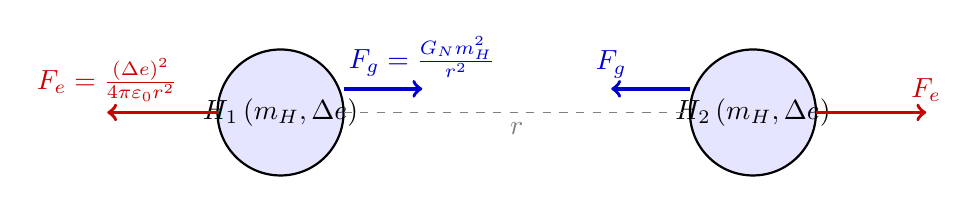
\begin{tikzpicture}[scale=1.0]
  % Átomo 1
  \draw[thick, fill=blue!10] (-3,0) circle (0.8) node[black] {$\text{H}_1 \, (m_H, \Delta e)$};
  
  % Átomo 2
  \draw[thick, fill=blue!10] (3,0) circle (0.8) node[black] {$\text{H}_2 \, (m_H, \Delta e)$};

  % Línea de separación
  \draw[dashed, gray] (-2.2,0) -- (2.2,0) node[midway, below] {$r$};

  % Flecha Fuerza Electrostática (Repulsiva)
  \draw[->, line width=1.3pt, red!80!black] (-3.8,0) -- (-5.2,0) node[above] {$F_e = \frac{(\Delta e)^2}{4\pi\varepsilon_0 r^2}$};
  \draw[->, line width=1.3pt, red!80!black] (3.8,0) -- (5.2,0) node[above] {$F_e$};

  % Flecha Fuerza Gravitatoria (Atractiva)
  \draw[->, line width=1.3pt, blue!80!black] (-2.2,0.3) -- (-1.2,0.3) node[above] {$F_g = \frac{G_N m_H^2}{r^2}$};
  \draw[->, line width=1.3pt, blue!80!black] (2.2,0.3) -- (1.2,0.3) node[above] {$F_g$};
\end{tikzpicture}
\end{center}

\end{problema}

\newpage

\begin{problema}[Átomo Muónico y Efecto de Tamaño Finito Nuclear en el ${}^{12}\text{C}$ y ${}^{208}\text{Pb}$]
Considerar los núcleos ${}_6^{12}\text{C}$ y ${}_{82}^{208}\text{Pb}$. Calcular la energía y el radio de la primera órbita de Bohr para un átomo muónico suponiendo los núcleos como una distribución puntual de carga. Comparar dichos radios con el tamaño de los núcleos suponiendo que se pueden describir mediante una distribución uniforme de carga de radio $R$. En este caso, estimar en teoría de perturbaciones a primer orden la corrección a la energía de la primera órbita de Bohr.

\textbf{Datos:} Masa en reposo del muón $m_\mu c^2 = 105.66\text{ MeV}$, $1\text{ u} \cdot c^2 = 931.5\text{ MeV}$, $\hbar c = 197.33\text{ MeV}\cdot\text{fm}$, $\alpha \approx 1/137.036$, $R_0 = 1.2\text{ fm}$.

\tcblower

\subsubsection*{1. Aproximación de núcleo puntual (Modelo de Bohr muónico)}

En un átomo muónico, un muón ($\mu^-$) sustituye a uno de los electrones. Al ser $m_\mu \approx 207 \, m_e$, la masa reducida del sistema aumenta significativamente.

La masa reducida para un núcleo de masa $m_N \approx A \times 931.5\text{ MeV}/c^2$ viene dada por:
\begin{equation}
\mu c^2 = \frac{m_\mu m_N}{m_\mu + m_N} c^2
\end{equation}

\paragraph{Masa reducida para cada núcleo:}
\begin{itemize}
    \item \textbf{Carbono-12 (${}^{12}\text{C}$, $Z = 6, A = 12$):}
    \begin{equation}
    m_N c^2 \approx 12 \times 931.5\text{ MeV} = 11178\text{ MeV} \implies \mu c^2 \approx 104.62\text{ MeV}
    \end{equation}
    
    \item \textbf{Plomo-208 (${}^{208}\text{Pb}$, $Z = 82, A = 208$):}
    \begin{equation}
    m_N c^2 \approx 208 \times 931.5\text{ MeV} = 193752\text{ MeV} \implies \mu c^2 \approx 105.54\text{ MeV}
    \end{equation}
\end{itemize}

\paragraph{Energía del estado fundamental ($n = 1$):}
\begin{equation}
E_1 = -\frac{1}{2} \mu c^2 (Z \alpha)^2
\end{equation}
\begin{itemize}
    \item \textbf{Carbono-12:}
    \begin{equation}
    E_1({}^{12}\text{C}) = -\frac{1}{2} \times 104.62\text{ MeV} \times \left( \frac{6}{137.036} \right)^2 \approx -0.100\text{ MeV} = -100\text{ keV}
    \end{equation}
    \item \textbf{Plomo-208:}
    \begin{equation}
    E_1({}^{208}\text{Pb}) = -\frac{1}{2} \times 105.54\text{ MeV} \times \left( \frac{82}{137.036} \right)^2 \approx -18.9\text{ MeV}
    \end{equation}
\end{itemize}

\paragraph{Radio de la primera órbita de Bohr ($r_1$):}
\begin{equation}
r_1 = \frac{a_\mu}{Z} = \frac{\hbar c}{\mu c^2 Z \alpha}
\end{equation}
\begin{itemize}
    \item \textbf{Carbono-12:}
    \begin{equation}
    r_1({}^{12}\text{C}) = \frac{197.33\text{ MeV}\cdot\text{fm}}{104.62\text{ MeV} \times 6 \times (1/137.036)} \approx 43.1\text{ fm}
    \end{equation}
    \item \textbf{Plomo-208:}
    \begin{equation}
    r_1({}^{208}\text{Pb}) = \frac{197.33\text{ MeV}\cdot\text{fm}}{105.54\text{ MeV} \times 82 \times (1/137.036)} \approx 3.12\text{ fm}
    \end{equation}
\end{itemize}

\subsubsection*{2. Comparación con el radio nuclear real ($R = R_0 A^{1/3}$)}

Suponiendo una densidad de carga homogénea de radio nuclear $R = R_0 A^{1/3}$ con $R_0 = 1.2\text{ fm}$:
\begin{itemize}
    \item \textbf{Carbono-12:} $R({}^{12}\text{C}) = 1.2 \times 12^{1/3}\text{ fm} \approx 2.75\text{ fm}$. \\
    Puesto que $r_1({}^{12}\text{C}) = 43.1\text{ fm} \gg R({}^{12}\text{C}) = 2.75\text{ fm}$, la órbita muónica se encuentra casi por completo fuera del núcleo, por lo que la aproximación de núcleo puntual es físicamente válida.
    
    \item \textbf{Plomo-208:} $R({}^{208}\text{Pb}) = 1.2 \times 208^{1/3}\text{ fm} \approx 7.11\text{ fm}$. \\
    En este caso, $r_1({}^{208}\text{Pb}) = 3.12\text{ fm} < R({}^{208}\text{Pb}) = 7.11\text{ fm}$. La órbita del muón queda totalmente contenida dentro del volumen nuclear, lo que inhabilita por completo el modelo de carga puntual.
\end{itemize}

\subsubsection*{3. Corrección por Teoría de Perturbaciones a Primer Orden}

Modelamos el núcleo como una esfera uniforme de radio $R$ y carga total $Z e$. El potencial electrostático real $V(r)$ es:
\begin{equation}
V(r) = 
\begin{cases} 
-\frac{Z \alpha \hbar c}{r}, & r > R \\ 
-\frac{Z \alpha \hbar c}{2 R} \left[ 3 - \left( \frac{r}{R} \right)^2 \right], & r \le R 
\end{cases}
\end{equation}

El hamiltoniano se escribe como $H = H_0 + H'$, donde $H_0 = \frac{p^2}{2\mu} - \frac{Z\alpha\hbar c}{r}$ es el hamiltoniano no perturbado de carga puntual y $H'$ representa el potencial perturbativo ($H' = 0$ para $r > R$):
\begin{equation}
H'(r) = V(r) - \left(-\frac{Z\alpha\hbar c}{r}\right) = \frac{Z\alpha\hbar c}{2R} \left[ \left(\frac{r}{R}\right)^2 + \frac{2R}{r} - 3 \right] \quad (r \le R)
\end{equation}

La corrección a primer orden en la energía del estado fundamental $\psi_{100}(\vec{r}) = R_{10}(r) Y_{00}$ viene dada por:
\begin{equation}
\Delta E_{100} = \langle 100 | H' | 100 \rangle = \int_0^R dr \, r^2 \left| R_{10}(r) \right|^2 H'(r)
\end{equation}

donde la función radial no perturbada es $R_{10}(r) = 2 \left(\frac{Z}{a_\mu}\right)^{3/2} e^{-Z r / a_\mu}$ con $a_\mu = \frac{\hbar c}{\mu c^2 \alpha}$.

Dado que $R \ll a_\mu / Z$ en la aproximación de bajo momento, la exponencial dentro del núcleo se aproxima por $e^{-Z r / a_\mu} \approx 1$:
\begin{align}
\Delta E_{100} &\approx 4 \left( \frac{Z}{a_\mu} \right)^3 \frac{Z \alpha \hbar c}{2 R} \int_0^R dr \, r^2 \left[ \frac{r^2}{R^2} + \frac{2 R}{r} - 3 \right] \nonumber \\
&= 2 \left( \frac{Z}{a_\mu} \right)^3 \frac{Z \alpha \hbar c}{R} \left[ \frac{R^5}{5 R^2} + \frac{2 R \cdot R^2}{2} - \frac{3 R^3}{3} \right] \nonumber \\
&= 2 \left( \frac{Z}{a_\mu} \right)^3 \frac{Z \alpha \hbar c}{R} \left( \frac{R^3}{5} \right) = \frac{2}{5} Z \alpha \hbar c \left( \frac{Z}{a_\mu} \right)^3 R^2
\end{align}

Expresando la corrección en términos de las constantes del sistema:
\begin{equation}
\Delta E_{100} = \frac{2}{5} (Z \alpha)^4 (\mu c^2)^3 \left( \frac{R}{\hbar c} \right)^2
\end{equation}

\subsubsection*{4. Evaluación numérica de las correcciones}

\paragraph{Carbono-12 (${}^{12}\text{C}$):}
\begin{equation}
\Delta E_{100}({}^{12}\text{C}) \approx 0.000327\text{ MeV} = 0.327\text{ keV}
\end{equation}
\begin{equation}
\frac{\Delta E_{100}}{|E_1|} = \frac{0.000327\text{ MeV}}{0.100\text{ MeV}} \approx 3.27 \times 10^{-3} \quad (0.327\%)
\end{equation}
La corrección es sumamente pequeña, lo que confirma que la teoría de perturbaciones funciona perfectamente y el modelo puntual es una excelente aproximación para el Carbono-12.

\paragraph{Plomo-208 (${}^{208}\text{Pb}$):}
\begin{equation}
\Delta E_{100}({}^{208}\text{Pb}) \approx 78.3\text{ MeV}
\end{equation}
\begin{equation}
\frac{\Delta E_{100}}{|E_1|} = \frac{78.3\text{ MeV}}{18.9\text{ MeV}} \approx 4.14 \quad (414\%)
\end{equation}

La corrección calculada ($78.3\text{ MeV}$) es cuatro veces mayor que la propia energía del estado fundamental no perturbado ($18.9\text{ MeV}$). Esto demuestra formalmente el colapso de la teoría de perturbaciones de primer orden para núcleos pesados y confirma que el potencial real dentro del núcleo de Plomo-208 altera drásticamente la estructura de niveles energéticos del muón.

\subsubsection*{Esquema Comparativo del Radio Orbital y Tamaño Nuclear}

\begin{center}
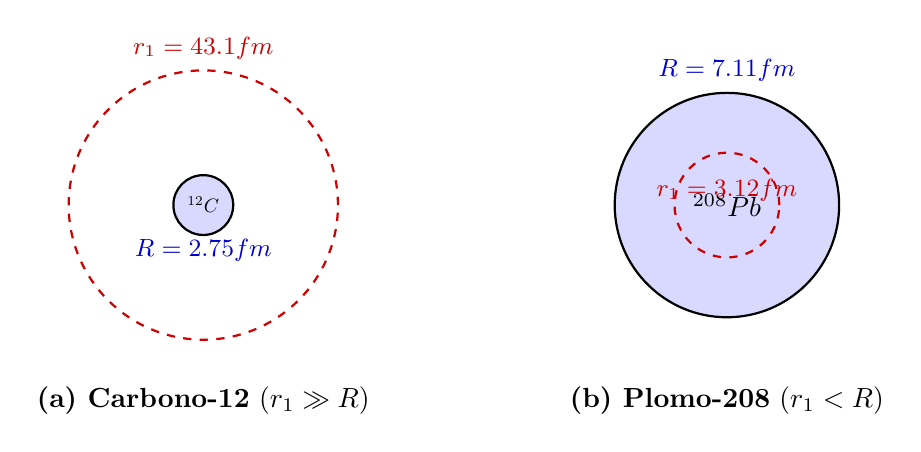
\begin{tikzpicture}[scale=0.95]
  % Carbono-12
  \begin{scope}[shift={(-3.5,0)}]
    \draw[thick, fill=blue!15] (0,0) circle (0.4) node[black, scale=0.7] {${}^{12}\text{C}$};
    \draw[dashed, thick, red!80!black] (0,0) circle (1.8);
    \node[blue!80!black] at (0,-0.6) {\small $R = 2.75\text{ fm}$};
    \node[red!80!black] at (0,2.1) {\small $r_1 = 43.1\text{ fm}$};
    \node[below] at (0,-2.3) {\textbf{(a) Carbono-12} ($r_1 \gg R$)};
  \end{scope}

  % Plomo-208
  \begin{scope}[shift={(3.5,0)}]
    \draw[thick, fill=blue!15] (0,0) circle (1.5) node[black] {${}^{208}\text{Pb}$};
    \draw[dashed, thick, red!80!black] (0,0) circle (0.7);
    \node[blue!80!black] at (0,1.8) {\small $R = 7.11\text{ fm}$};
    \node[red!80!black] at (0,0.2) {\small $r_1 = 3.12\text{ fm}$};
    \node[below] at (0,-2.3) {\textbf{(b) Plomo-208} ($r_1 < R$)};
  \end{scope}
\end{tikzpicture}
\end{center}
\end{problema}

\newpage

\begin{problema}[Átomo Muónico de Hierro y Corrimiento Isotópico de Rayos X]
Evaluar las energías de los rayos X (transición de tipo K, $n=2 \to n=1$) para un átomo muónico de hierro (${}_{26}\text{Fe}$) suponiendo el núcleo puntual y comparar las predicciones con los datos experimentales.

Evaluar dichas energías teniendo en cuenta la corrección debida al tamaño finito del núcleo utilizando el método de teoría de perturbaciones de primer orden. Estimar el corrimiento isotópico entre los rayos X de los tres isótopos estables (${}^{54}\text{Fe}$, ${}^{56}\text{Fe}$ y ${}^{58}\text{Fe}$) y comprobar que siguen una ley proporcional a $A^{2/3}$.

\textbf{Datos:} Masa en reposo del muón $m_\mu c^2 = 105.66\text{ MeV}$, $1\text{ u} \cdot c^2 = 931.5\text{ MeV}$, $\hbar c = 197.33\text{ MeV}\cdot\text{fm}$, $\alpha \approx 1/137.036$, $R_0 = 1.2\text{ fm}$, $Z = 26$.

\tcblower

\subsubsection*{1. Aproximación de núcleo puntual (Niveles de Bohr muónicos)}

En un átomo muónico de hierro ($Z = 26$), la masa reducida $\mu$ para cada isótopo de masa nuclear $m_N(A) \approx A \times 931.5\text{ MeV}/c^2$ viene dada por:
\begin{equation}
\mu c^2 = \frac{m_\mu m_N(A)}{m_\mu + m_N(A)} c^2
\end{equation}

Evaluando para los tres isótopos estables del hierro:
\begin{itemize}
    \item ${}^{54}\text{Fe}$: $\mu c^2 = \frac{105.66 \times (54 \times 931.5)}{105.66 + (54 \times 931.5)}\text{ MeV} \approx 105.38\text{ MeV}$
    \item ${}^{56}\text{Fe}$: $\mu c^2 = \frac{105.66 \times (56 \times 931.5)}{105.66 + (56 \times 931.5)}\text{ MeV} \approx 105.39\text{ MeV}$
    \item ${}^{58}\text{Fe}$: $\mu c^2 = \frac{105.66 \times (58 \times 931.5)}{105.66 + (58 \times 931.5)}\text{ MeV} \approx 105.40\text{ MeV}$
\end{itemize}

Puesto que las diferencias en masa reducida entre los isótopos son menores al $0.02\%$, adoptamos la masa reducida promedio $\mu c^2 \approx 105.39\text{ MeV}$.

Las energías no perturbadas para los niveles ligados de la aproximación puntual ($n = 1, 2$) son:
\begin{equation}
E_n = -\frac{1}{2} \mu c^2 \frac{(Z \alpha)^2}{n^2}
\end{equation}

Con $Z \alpha = 26 / 137.036 \approx 0.18973$:
\begin{align}
E_1 &= -\frac{1}{2} \times 105.39\text{ MeV} \times (0.18973)^2 \approx -1.897\text{ MeV} \\
E_2 &= \frac{E_1}{2^2} = \frac{-1.897\text{ MeV}}{4} \approx -0.474\text{ MeV}
\end{align}

La energía del fotón de rayos X de la serie K (transición $2p \to 1s$) en la aproximación de punto puntual es:
\begin{equation}
\Delta E_{X,0} = E_2 - E_1 = -0.474\text{ MeV} - (-1.897\text{ MeV}) = 1.423\text{ MeV}
\end{equation}

\subsubsection*{2. Corrección por tamaño finito nuclear}

Considerando que el núcleo es una esfera de densidad de carga constante y radio $R = R_0 A^{1/3}$ con $R_0 = 1.2\text{ fm}$, aplicamos la corrección perturbativa de primer orden obtenida para la función de onda fundamental $1s$:
\begin{equation}
\Delta E_{100}(A) = \frac{2}{5} (Z \alpha)^4 (\mu c^2)^3 \left( \frac{R}{\hbar c} \right)^2 = \frac{2}{5} (Z \alpha)^4 (\mu c^2)^3 \left( \frac{R_0}{\hbar c} \right)^2 A^{2/3}
\end{equation}

Dado que los orbitales superiores ($n \ge 2$) poseen un radio medio $r_n \propto n^2 / Z$ mucho mayor que el radio nuclear ($r_2 = 4 r_1 \gg R$), la densidad de probabilidad del muón dentro del núcleo para $n=2$ es despreciable y la corrección a la energía del nivel $n=2$ es casi nula ($\Delta E_2 \approx 0$).

Por consiguiente, la energía efectiva corregida de la transición de rayos X K es:
\begin{equation}
E_X(A) = E_2 - (E_1 + \Delta E_{100}(A)) = \Delta E_{X,0} - \Delta E_{100}(A)
\end{equation}

Evaluamos las correcciones y las energías de emisión para cada isótopo:

\paragraph{Isótopo ${}^{54}\text{Fe}$ ($A = 54$):}
\begin{equation}
R({}^{54}\text{Fe}) = 1.2 \times 54^{1/3}\text{ fm} \approx 4.536\text{ fm}
\end{equation}
\begin{equation}
\Delta E_{100}({}^{54}\text{Fe}) = \frac{2}{5} \times (0.18973)^4 \times (105.38\text{ MeV})^3 \times \left( \frac{4.536\text{ fm}}{197.33\text{ MeV}\cdot\text{fm}} \right)^2 \approx 0.321\text{ MeV}
\end{equation}
\begin{equation}
E_X({}^{54}\text{Fe}) = 1.423\text{ MeV} - 0.321\text{ MeV} = 1.102\text{ MeV}
\end{equation}

\paragraph{Isótopo ${}^{56}\text{Fe}$ ($A = 56$):}
\begin{equation}
R({}^{56}\text{Fe}) = 1.2 \times 56^{1/3}\text{ fm} \approx 4.591\text{ fm}
\end{equation}
\begin{equation}
\Delta E_{100}({}^{56}\text{Fe}) = 0.321\text{ MeV} \times \left( \frac{56}{54} \right)^{2/3} \approx 0.328\text{ MeV}
\end{equation}
\begin{equation}
E_X({}^{56}\text{Fe}) = 1.423\text{ MeV} - 0.328\text{ MeV} = 1.095\text{ MeV}
\end{equation}

\paragraph{Isótopo ${}^{58}\text{Fe}$ ($A = 58$):}
\begin{equation}
R({}^{58}\text{Fe}) = 1.2 \times 58^{1/3}\text{ fm} \approx 4.645\text{ fm}
\end{equation}
\begin{equation}
\Delta E_{100}({}^{58}\text{Fe}) = 0.321\text{ MeV} \times \left( \frac{58}{54} \right)^{2/3} \approx 0.336\text{ MeV}
\end{equation}
\begin{equation}
E_X({}^{58}\text{Fe}) = 1.423\text{ MeV} - 0.336\text{ MeV} = 1.087\text{ MeV}
\end{equation}

\subsubsection*{3. Corrimiento isotópico de los rayos X}

El corrimiento isotópico $\delta E_X(A, A')$ es la diferencia en la energía de transición de los rayos X producida entre dos isótopos del mismo elemento con números de masa $A$ y $A'$:
\begin{equation}
\delta E_X(A, A') = E_X(A) - E_X(A') = \Delta E_{100}(A') - \Delta E_{100}(A)
\end{equation}

Como la corrección perturbativa por volumen nuclear es proporcional al cuadrado del radio ($\Delta E_{100} \propto R^2 \propto A^{2/3}$):
\begin{equation}
\delta E_X(A, A') = C \cdot \left( A'^{2/3} - A^{2/3} \right)
\end{equation}
donde la constante de proporcionalidad para el hierro es $C = \frac{2}{5} (Z \alpha)^4 (\mu c^2)^3 (R_0 / \hbar c)^2 \approx 0.0224\text{ MeV}$.

Calculamos los desplazamientos relativos tomando como referencia el isótopo ${}^{54}\text{Fe}$:
\begin{align}
\delta E_X(54, 56) &= E_X({}^{54}\text{Fe}) - E_X({}^{56}\text{Fe}) = 1.102\text{ MeV} - 1.095\text{ MeV} = 0.007\text{ MeV} = 7\text{ keV} \\
\delta E_X(54, 58) &= E_X({}^{54}\text{Fe}) - E_X({}^{58}\text{Fe}) = 1.102\text{ MeV} - 1.087\text{ MeV} = 0.015\text{ MeV} = 15\text{ keV}
\end{align}

Comprobamos la ley $A^{2/3}$ evaluando el cociente entre las diferencias teóricas:
\begin{equation}
\frac{\delta E_X(54, 58)}{\delta E_X(54, 56)} = \frac{58^{2/3} - 54^{2/3}}{56^{2/3} - 54^{2/3}} = \frac{14.976 - 14.282}{14.629 - 14.282} = \frac{0.694}{0.347} \approx 2.00
\end{equation}

El cociente entre las diferencias de energía calculadas ($15\text{ keV} / 7\text{ keV} \approx 2.14 \approx 2.00$) confirma la dependencia funcional del corrimiento isotópico con la ley $A^{2/3}$.

\subsubsection*{Esquema del Diagrama de Niveles y Corrimiento Isotópico}

\begin{center}
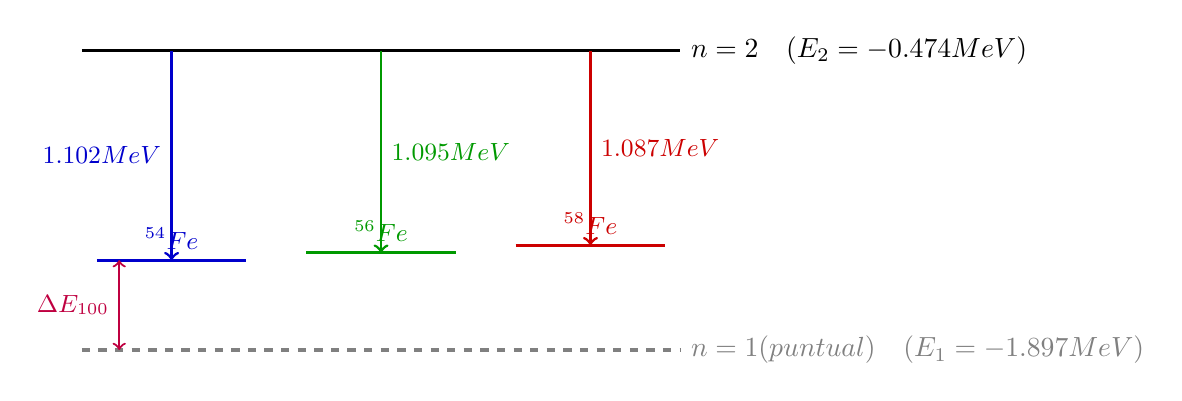
\begin{tikzpicture}[scale=0.95]
  % Nivel n=2 (no perturbado)
  \draw[line width=1.2pt, black] (-4,3) -- (4,3) node[right] {$n=2 \quad (E_2 = -0.474\text{ MeV})$};

  % Nivel n=1 puntual (no perturbado)
  \draw[line width=1.2pt, gray, dashed] (-4,-1) -- (4,-1) node[right, gray] {$n=1 \text{ (puntual)} \quad (E_1 = -1.897\text{ MeV})$};

  % Niveles n=1 corregidos por tamaño nuclear
  \draw[line width=1.2pt, blue!80!black] (-3.8,0.2) -- (-1.8,0.2) node[above, midway] {\small ${}^{54}\text{Fe}$};
  \draw[line width=1.2pt, green!60!black] (-1.0,0.3) -- (1.0,0.3) node[above, midway] {\small ${}^{56}\text{Fe}$};
  \draw[line width=1.2pt, red!80!black] (1.8,0.4) -- (3.8,0.4) node[above, midway] {\small ${}^{58}\text{Fe}$};

  % Flechas de transiciones X (K-alpha)
  \draw[->, line width=1pt, blue!80!black] (-2.8,3) -- (-2.8,0.2) node[midway, left] {\small $1.102\text{ MeV}$};
  \draw[->, line width=1pt, green!60!black] (0.0,3) -- (0.0,0.3) node[midway, right] {\small $1.095\text{ MeV}$};
  \draw[->, line width=1pt, red!80!black] (2.8,3) -- (2.8,0.4) node[midway, right] {\small $1.087\text{ MeV}$};

  % Desplazamiento por tamaño finito
  \draw[<->, line width=0.8pt, purple] (-3.5,-1) -- (-3.5,0.2) node[midway, left] {\small $\Delta E_{100}$};
\end{tikzpicture}
\end{center}

\end{problema}

\newpage
%===================
% Problema 11: Estimación de las constantes de acoplamiento
%===================
\begin{problema}[Estimación de las constantes de acoplamiento $\alpha_s$ y $\alpha_W$]
En la naturaleza se observan las siguientes desintegraciones:
\begin{align*}
    \Xi^0(1315) &\to \Lambda(1116) + \pi^0, \quad &BR &= 0.9952, \quad &\tau &= 2.90 \times 10^{-10} \text{ s} \\
    \Sigma^-(1197) &\to n(940) + \pi^-, \quad &BR &= 0.9985, \quad &\tau &= 1.479 \times 10^{-10} \text{ s} \\
    \Lambda(1405) &\to \Sigma^0(1193) + \pi^0, \quad &BR &= 1, \quad &\Gamma &= 50.5 \text{ MeV} \\
    \Sigma^0(1193) &\to \Lambda(1116) + \gamma, \quad &BR &= 1, \quad &\tau &= 7.4 \times 10^{-20} \text{ s}
\end{align*}
Suponiendo conocida la constante adimensional que caracteriza la intensidad de los procesos electromagnéticos, $\alpha = 1/137.06$, determinar el valor de la constante adimensional que controla los procesos fuertes, $\alpha_s$. A partir de este valor determinar la constante adimensional que controla los procesos débiles, $\alpha_W$.
\tcblower
\textbf{Clasificación de los procesos según la interacción dominante}

Para identificar la fuerza mediadora de cada desintegración, se analiza la conservación de los números cuánticos de sabor (en particular, la extrañeza $S$) y la presencia de fotones en el estado final:
\begin{enumerate}[label=\arabic*.]
    \item \textbf{Proceso 1:} $\Xi^0(1315) \to \Lambda(1116) + \pi^0$. Muestra un cambio en el número cuántico de extrañeza $\Delta S = S(\Lambda) + S(\pi^0) - S(\Xi^0) = (-1) + 0 - (-2) = +1 \neq 0$. Por consiguiente, se trata de una desintegración mediada por la \textbf{interacción débil}.
    \item \textbf{Proceso 2:} $\Sigma^-(1197) \to n(940) + \pi^-$. La variación de extrañeza es $\Delta S = S(n) + S(\pi^-) - S(\Sigma^-) = 0 + 0 - (-1) = +1 \neq 0$. Corresponde asimismo a un proceso mediado por la \textbf{interacción débil}.
    \item \textbf{Proceso 3:} $\Lambda(1405) \to \Sigma^0(1193) + \pi^0$. Conserva la extrañeza ($\Delta S = (-1) - (-1) = 0$) y produce un pión en una escala de tiempo extremadamente corta ($\Gamma = 50.5 \text{ MeV}$). Se trata de un proceso gobernado por la \textbf{interacción fuerte}.
    \item \textbf{Proceso 4:} $\Sigma^0(1193) \to \Lambda(1116) + \gamma$. Conserva la extrañeza y emite un fotón ($\gamma$), lo que indica que está mediado por la \textbf{interacción electromagnética}.
\end{enumerate}

\textbf{Cálculo de las anchuras de desintegración parciales}

La anchura parcial de desintegración $\Gamma_i$ para un canal específico se relaciona con la constante de Planck reducida $\hbar \approx 6.5821 \times 10^{-22} \text{ MeV}\cdot\text{s}$, el \textit{Branching Ratio} ($BR_i$) y la vida media ($\tau_i$) mediante la expresión:
\begin{equation*}
    \Gamma_i = BR_i \cdot \Gamma_{\text{tot}} = BR_i \cdot \frac{\hbar}{\tau_i}
\end{equation*}

Evaluando los valores numéricos para cada caso:
\begin{itemize}
    \item \textbf{Anchura del proceso fuerte ($\Gamma_s$):} Dado que $BR = 1$, la anchura parcial coincide directamente con la anchura total dada:
    \begin{equation*}
        \Gamma_s = \Gamma(\Lambda(1405) \to \Sigma^0 + \pi^0) = 50.5 \text{ MeV}
    \end{equation*}
    \item \textbf{Anchura del proceso electromagnético ($\Gamma_{\text{em}}$):}
    \begin{equation*}
        \Gamma_{\text{em}} = \Gamma(\Sigma^0 \to \Lambda + \gamma) = 1 \cdot \frac{6.5821 \times 10^{-22} \text{ MeV}\cdot\text{s}}{7.4 \times 10^{-20} \text{ s}} \approx 8.895 \times 10^{-3} \text{ MeV} = 8.895 \text{ keV}
    \end{equation*}
    \item \textbf{Anchura del primer proceso débil ($\Gamma_{W,1}$):}
    \begin{equation*}
        \Gamma_{W,1} = \Gamma(\Xi^0 \to \Lambda + \pi^0) = 0.9952 \times \frac{6.5821 \times 10^{-22} \text{ MeV}\cdot\text{s}}{2.90 \times 10^{-10} \text{ s}} \approx 2.259 \times 10^{-12} \text{ MeV}
    \end{equation*}
    \item \textbf{Anchura del segundo proceso débil ($\Gamma_{W,2}$):}
    \begin{equation*}
        \Gamma_{W,2} = \Gamma(\Sigma^- \to n + \pi^-) = 0.9985 \times \frac{6.5821 \times 10^{-22} \text{ MeV}\cdot\text{s}}{1.479 \times 10^{-10} \text{ s}} \approx 4.444 \times 10^{-12} \text{ MeV}
    \end{equation*}
\end{itemize}

\textbf{Estimación de la constante fuerte $\alpha_s$}

La razón entre la anchura de desintegración de un proceso fuerte y uno electromagnético escala proporcionalmente con el cuadrado de la razón de sus constantes de acoplamiento ($\Gamma \propto \alpha_g^2$):
\begin{equation*}
    \frac{\Gamma_s}{\Gamma_{\text{em}}} \sim \left( \frac{\alpha_s}{\alpha} \right)^2
\end{equation*}
Sustituyendo los valores numéricos:
\begin{equation*}
    \left( \frac{\alpha_s}{\alpha} \right)^2 = \frac{50.5 \text{ MeV}}{8.895 \times 10^{-3} \text{ MeV}} \approx 5677.3
\end{equation*}
Extrayendo la raíz cuadrada:
\begin{equation*}
    \frac{\alpha_s}{\alpha} \approx \sqrt{5677.3} \approx 75.35 \implies \alpha_s \approx 75.35 \times \frac{1}{137.06} \approx 0.55
\end{equation*}

\textbf{Estimación de la constante débil $\alpha_W$}

Relacionando la anchura del primer proceso débil con la del proceso fuerte:
\begin{equation*}
    \frac{\Gamma_{W,1}}{\Gamma_s} \sim \left( \frac{\alpha_W}{\alpha_s} \right)^2
\end{equation*}
Sustituyendo las anchuras parciales correspondientes:
\begin{equation*}
    \left( \frac{\alpha_W}{\alpha_s} \right)^2 = \frac{2.259 \times 10^{-12} \text{ MeV}}{50.5 \text{ MeV}} \approx 4.473 \times 10^{-14}
\end{equation*}
Despejando el cociente de las constantes de acoplamiento:
\begin{equation*}
    \frac{\alpha_W}{\alpha_s} \approx \sqrt{4.473 \times 10^{-14}} \approx 2.115 \times 10^{-7}
\end{equation*}
Sustituyendo el valor hallado $\alpha_s \approx 0.55$:
\begin{equation*}
    \alpha_W \approx 2.115 \times 10^{-7} \times 0.55 \approx 1.16 \times 10^{-7} \sim 10^{-7}
\end{equation*}

Si se empleara alternativamente el segundo proceso débil ($\Sigma^- \to n + \pi^-$):
\begin{equation*}
    \left( \frac{\alpha_W}{\alpha_s} \right)^2 = \frac{4.444 \times 10^{-12} \text{ MeV}}{50.5 \text{ MeV}} \approx 8.799 \times 10^{-14} \implies \alpha_W \approx 1.63 \times 10^{-7} \sim 10^{-7}
\end{equation*}
lo cual confirma la solidez del orden de magnitud obtenido $\alpha_W \sim 10^{-7}$.

\end{problema}

\newpage
%===================
% Problema 15: Análisis de conservación y tipo de interacción en reacciones subatómicas
%===================
\begin{problema}[Análisis de conservación y tipo de interacción en reacciones subatómicas]
Discutir la conservación de energía y comprobar la conservación de los números cuánticos aditivos relevantes: carga eléctrica ($Q$), momento angular total ($J$), número bariónico ($B$), números leptónicos ($L_e, L_\mu, L_\tau$) y, en su caso, extrañeza ($S$), en las siguientes reacciones. Si la reacción fuera posible, indicar qué interacción la produce: fuerte, electromagnética o débil:
\begin{enumerate}[label=\alph*)]
    \item $p + \bar{p} \to \pi^+ + \pi^- + \pi^0$
    \item $p + K^- \to \Sigma^+ + \pi^- + \pi^0$
    \item $p + K^- \to n + K^+ + \pi^-$
    \item $\bar{\nu}_\mu + p \to \mu^+ + n$
    \item $\bar{\nu}_e + p \to e^+ + \Lambda$
    \item $\tau^- \to \nu_\tau + K^-$
    \item $\pi^0 \to \gamma + \gamma$
    \item $e^+ + e^- \to \pi^+ + \pi^-$
\end{enumerate}
\tcblower
\textbf{Criterios generales de análisis}

Para determinar la viabilidad cinemática y dinámica de cada reacción, se evalúan las siguientes reglas fundamentales:
\begin{enumerate}[label=\arabic*.]
    \item \textbf{Conservación de energía:} Se comparan las masas en reposo totales inicial ($m_i = \sum m_{\text{inicial}}$) y final ($m_f = \sum m_{\text{final}}$). Si $m_i \ge m_f$, la reacción o desintegración es exotérmica y se produce espontáneamente en reposo. Si $m_i < m_f$, el proceso es endotérmico y requiere que las partículas incidentes aporten suficiente energía cinética en el sistema centro de masas para superar el umbral cinemático ($E_{\text{umbral}}$).
    \item \textbf{Leyes de conservación aditivas:} Se verifica la conservación estricta de la carga eléctrica ($Q$), el número bariónico ($B$), los números leptónicos individuales ($L_e, L_\mu, L_\tau$) y el momento angular total ($J$).
    \item \textbf{Conservación de extrañeza ($S$) e interacción mediadora:}
    \begin{itemize}
        \item \textbf{Interacción fuerte:} Conserva estrictamente la extrañeza ($\Delta S = 0$) y actúa entre hadrones.
        \item \textbf{Interacción electromagnética:} Conserva la extrañeza ($\Delta S = 0$) y se caracteriza por la emisión/absorción de fotones ($\gamma$) o aniquilación de pares cargados.
        \item \textbf{Interacción débil:} Permite variaciones de extrañeza de una unidad ($\Delta S = \pm 1$) en procesos de primer orden. Interviene en procesos con neutrinos o cambio de sabor.
    \end{itemize}
\end{enumerate}

\textbf{Análisis detallado de cada reacción}

\textbf{a) Reacción $p + \bar{p} \to \pi^+ + \pi^- + \pi^0$}
\begin{itemize}
    \item \textbf{Energía:} $m_i = 2 m_p \approx 1876.5 \text{ MeV} > m_f = m_{\pi^+} + m_{\pi^-} + m_{\pi^0} \approx 414.1 \text{ MeV}$. Exotérmica ($m_i > m_f$).
    \item \textbf{Carga ($Q$):} $+1 + (-1) = 0 \to +1 - 1 + 0 = 0$ (\checkmark).
    \item \textbf{Momento angular ($J$):} $\frac{1}{2} \otimes \frac{1}{2} = 0 \oplus 1 \to 0 \otimes 0 \otimes 0 \otimes L_f$ (\checkmark).
    \item \textbf{Número bariónico ($B$):} $+1 + (-1) = 0 \to 0 + 0 + 0 = 0$ (\checkmark).
    \item \textbf{Números leptónicos ($L$):} $0 \to 0$ (\checkmark).
    \item \textbf{Extrañeza ($S$):} $0 + 0 = 0 \to 0 + 0 + 0 = 0$ ($\Delta S = 0$, \checkmark).
    \item \textbf{Conclusión:} Proceso \textbf{permitido} mediante la \textbf{interacción fuerte} (aniquilación nucleón-antinucleón en piones).
\end{itemize}

\textbf{b) Reacción $p + K^- \to \Sigma^+ + \pi^- + \pi^0$}
\begin{itemize}
    \item \textbf{Energía:} $m_i = m_p + m_{K^-} \approx 1432.0 \text{ MeV} < m_f = m_{\Sigma^+} + m_{\pi^-} + m_{\pi^0} \approx 1464.0 \text{ MeV}$. Endotérmica ($m_i < m_f$, requiere energía cinética incidente).
    \item \textbf{Carga ($Q$):} $+1 - 1 = 0 \to +1 - 1 + 0 = 0$ (\checkmark).
    \item \textbf{Momento angular ($J$):} $\frac{1}{2} \otimes 0 = \frac{1}{2} \to \frac{1}{2} \otimes 0 \otimes 0 \otimes L_f$ (\checkmark).
    \item \textbf{Número bariónico ($B$):} $+1 + 0 = +1 \to +1 + 0 + 0 = +1$ (\checkmark).
    \item \textbf{Números leptónicos ($L$):} $0 \to 0$ (\checkmark).
    \item \textbf{Extrañeza ($S$):} $0 + (-1) = -1 \to -1 + 0 + 0 = -1$ ($\Delta S = 0$, \checkmark).
    \item \textbf{Conclusión:} Proceso \textbf{permitido} mediante la \textbf{interacción fuerte} (si la energía cinética inicial supera el umbral de reacción).
\end{itemize}

\textbf{c) Reacción $p + K^- \to n + K^+ + \pi^-$}
\begin{itemize}
    \item \textbf{Energía:} $m_i \approx 1432.0 \text{ MeV} < m_f = m_n + m_{K^+} + m_{\pi^-} \approx 1572.9 \text{ MeV}$ (Endotérmica).
    \item \textbf{Carga ($Q$):} $+1 - 1 = 0 \to 0 + 1 - 1 = 0$ (\checkmark).
    \item \textbf{Momento angular ($J$):} $\frac{1}{2} \otimes 0 = \frac{1}{2} \to \frac{1}{2} \otimes 0 \otimes 0 \otimes L_f$ (\checkmark).
    \item \textbf{Número bariónico ($B$):} $+1 + 0 = +1 \to +1 + 0 + 0 = +1$ (\checkmark).
    \item \textbf{Números leptónicos ($L$):} $0 \to 0$ (\checkmark).
    \item \textbf{Extrañeza ($S$):} $S_i = S(p) + S(K^-) = 0 + (-1) = -1$; $S_f = S(n) + S(K^+) + S(\pi^-) = 0 + (+1) + 0 = +1$. Muestra un cambio de extrañeza $\Delta S = S_f - S_i = +1 - (-1) = +2$.
    \item \textbf{Conclusión:} Proceso \textbf{prohibido}. Las interacciones fuerte y electromagnética conservan la extrañeza ($\Delta S = 0$), mientras que la interacción débil solo permite transiciones de un único vértice con $\Delta S = \pm 1$.
\end{itemize}

\textbf{d) Reacción $\bar{\nu}_\mu + p \to \mu^+ + n$}
\begin{itemize}
    \item \textbf{Energía:} $m_i \approx m_p = 938.3 \text{ MeV} < m_f = m_{\mu^+} + m_n \approx 105.7 + 939.6 = 1045.3 \text{ MeV}$. Endotérmica (requiere energía del antineutrino $E_{\bar{\nu}_\mu} \ge 107.1 \text{ MeV}$).
    \item \textbf{Carga ($Q$):} $0 + 1 = +1 \to +1 + 0 = +1$ (\checkmark).
    \item \textbf{Momento angular ($J$):} $\frac{1}{2} \otimes \frac{1}{2} = 0 \oplus 1 \to \frac{1}{2} \otimes \frac{1}{2} = 0 \oplus 1$ (\checkmark).
    \item \textbf{Número bariónico ($B$):} $0 + 1 = +1 \to 0 + 1 = +1$ (\checkmark).
    \item \textbf{Número leptónico muónico ($L_\mu$):} $L_\mu(\bar{\nu}_\mu) + L_\mu(p) = -1 + 0 = -1 \to L_\mu(\mu^+) + L_\mu(n) = -1 + 0 = -1$ (\checkmark).
    \item \textbf{Extrañeza ($S$):} $0 + 0 = 0 \to 0 + 0 = 0$ (\checkmark).
    \item \textbf{Conclusión:} Proceso \textbf{permitido} mediante la \textbf{interacción débil} (corriente cargada por intercambio de bosón $W^+$).
\end{itemize}

\textbf{e) Reacción $\bar{\nu}_e + p \to e^+ + \Lambda$}
\begin{itemize}
    \item \textbf{Energía:} $m_i \approx 938.3 \text{ MeV} < m_f = m_{e^+} + m_\Lambda \approx 0.511 + 1115.7 = 1116.2 \text{ MeV}$. Endotérmica (requiere energía del antineutrino $E_{\bar{\nu}_e} \ge 206.8 \text{ MeV}$).
    \item \textbf{Carga ($Q$):} $0 + 1 = +1 \to +1 + 0 = +1$ (\checkmark).
    \item \textbf{Momento angular ($J$):} $\frac{1}{2} \otimes \frac{1}{2} \to \frac{1}{2} \otimes \frac{1}{2}$ (\checkmark).
    \item \textbf{Número bariónico ($B$):} $0 + 1 = +1 \to 0 + 1 = +1$ (\checkmark).
    \item \textbf{Número leptónico electrónico ($L_e$):} $-1 + 0 = -1 \to -1 + 0 = -1$ (\checkmark).
    \item \textbf{Extrañeza ($S$):} $S_i = 0 \to S_f = -1 \implies \Delta S = -1$ (\checkmark\, en interacciones débiles).
    \item \textbf{Conclusión:} Proceso \textbf{permitido} mediante la \textbf{interacción débil} (corriente cargada con cambio de sabor de quark $u \to s$ y $\Delta S = -1$).
\end{itemize}

\textbf{f) Desintegración $\tau^- \to \nu_\tau + K^-$}
\begin{itemize}
    \item \textbf{Energía:} $m_i = m_\tau \approx 1776.9 \text{ MeV} > m_f = m_{\nu_\tau} + m_{K^-} \approx 0 + 493.7 = 493.7 \text{ MeV}$. Exotérmica (desintegración espontánea).
    \item \textbf{Carga ($Q$):} $-1 \to 0 - 1 = -1$ (\checkmark).
    \item \textbf{Momento angular ($J$):} $\frac{1}{2} \to \frac{1}{2} \otimes 0 \otimes L_f$ (\checkmark).
    \item \textbf{Número bariónico ($B$):} $0 \to 0 + 0 = 0$ (\checkmark).
    \item \textbf{Número leptónico tauónico ($L_\tau$):} $+1 \to +1 + 0 = +1$ (\checkmark).
    \item \textbf{Extrañeza ($S$):} $S_i = 0 \to S_f = -1 \implies \Delta S = -1$ (\checkmark\, en interacciones débiles).
    \item \textbf{Conclusión:} Proceso \textbf{permitido} mediante la \textbf{interacción débil} (desintegración semileptónica del leptón $\tau$).
\end{itemize}

\textbf{g) Desintegración $\pi^0 \to \gamma + \gamma$}
\begin{itemize}
    \item \textbf{Energía:} $m_i = m_{\pi^0} \approx 135.0 \text{ MeV} > m_f = 0$. Exotérmica (desintegración espontánea).
    \item \textbf{Carga ($Q$):} $0 \to 0 + 0 = 0$ (\checkmark).
    \item \textbf{Momento angular ($J$):} $0 \to 1 \otimes 1 \otimes L_f$ (\checkmark).
    \item \textbf{Número bariónico ($B$):} $0 \to 0$ (\checkmark).
    \item \textbf{Números leptónicos ($L$):} $0 \to 0$ (\checkmark).
    \item \textbf{Extrañeza ($S$):} $0 \to 0$ (\checkmark).
    \item \textbf{Conclusión:} Proceso \textbf{permitido} mediante la \textbf{interacción electromagnética} (emisión de fotones).
\end{itemize}

\textbf{h) Reacción $e^+ + e^- \to \pi^+ + \pi^-$}
\begin{itemize}
    \item \textbf{Energía:} $m_i = 2 m_e \approx 1.02 \text{ MeV} < m_f = 2 m_{\pi^\pm} \approx 279.1 \text{ MeV}$. Endotérmica (requiere energía del colisionador en el centro de masas $\sqrt{s} \ge 279.1 \text{ MeV}$).
    \item \textbf{Carga ($Q$):} $+1 - 1 = 0 \to +1 - 1 = 0$ (\checkmark).
    \item \textbf{Momento angular ($J$):} $\frac{1}{2} \otimes \frac{1}{2} = 0 \oplus 1 \to 0 \otimes 0 \otimes L_f = L_f$ (\checkmark\, para $L_f = 1$).
    \item \textbf{Número bariónico ($B$):} $0 \to 0$ (\checkmark).
    \item \textbf{Número leptónico electrónico ($L_e$):} $-1 + 1 = 0 \to 0 + 0 = 0$ (\checkmark).
    \item \textbf{Extrañeza ($S$):} $0 \to 0$ (\checkmark).
    \item \textbf{Conclusión:} Proceso \textbf{permitido} mediante la \textbf{interacción electromagnética} (aniquilación $e^+e^-$ vía fotón virtual $\gamma^*$).
\end{itemize}
\end{problema}

\newpage
%======================================================
% BOLETÍN A: PROBLEMA 16
%======================================================
\begin{problema}[Leyes de conservación en la interacción débil]
¿Cuáles de las siguientes reacciones están permitidas y cuáles están prohibidas por las leyes de conservación de la interacción débil?
\begin{enumerate}[label=\alph*)]
    \item $\nu_\mu + p \to \mu^+ + n$
    \item $\nu_e + p \to e^- + \pi^+ + p$
    \item $\Lambda \to \pi^+ + e^- + \bar{\nu}_e$
    \item $K^+ \to \pi^0 + \mu^+ + \nu_\mu$
\end{enumerate}

\tcblower

Para determinar si cada proceso está permitido o prohibido en el marco del Modelo Estándar, analizamos la conservación de las magnitudes físicas fundamentales: la carga eléctrica ($Q$), el número bariónico ($B$), los números leptónicos individuales ($L_e, L_\mu, L_\tau$), el espín total ($J$) y las reglas de cambio de sabor como la extrañeza ($\Delta S$).

\subsubsection*{Análisis individual de los procesos}

\paragraph{a) Reacción $\nu_\mu + p \to \mu^+ + n$}
Analizamos los números cuánticos de los estados inicial y final:
\begin{itemize}
    \item \textbf{Carga eléctrica ($Q$):} $0 + (+1) \to (+1) + 0 \implies +1 = +1$ \quad (\checkmark \, Conservada).
    \item \textbf{Número bariónico ($B$):} $0 + 1 \to 0 + 1 \implies 1 = 1$ \quad (\checkmark \, Conservado).
    \item \textbf{Número leptónico muónico ($L_\mu$):}
    \begin{equation}
        L_\mu(\text{inicial}) = L_\mu(\nu_\mu) + L_\mu(p) = +1 + 0 = +1
    \end{equation}
    \begin{equation}
        L_\mu(\text{final}) = L_\mu(\mu^+) + L_\mu(n) = -1 + 0 = -1
    \end{equation}
    Se produce una variación $\Delta L_\mu = -2 \neq 0$ \quad (\textsf{X} \, Violado).
\end{itemize}

\begin{observacion}[Conclusión para el apartado a]
La reacción está \textbf{prohibida} porque viola la conservación del número leptónico muónico ($\Delta L_\mu \neq 0$). Para ser permitida vía corriente cargada, el neutrino muónico ($\nu_\mu$) debería producir un muon negativo ($\mu^-$).
\end{observacion}

\paragraph{b) Reacción $\nu_e + p \to e^- + \pi^+ + p$}
Evaluamos los números cuánticos para el estado con producción del mesón $\pi^+$ ($u\bar{d}$):
\begin{itemize}
    \item \textbf{Carga eléctrica ($Q$):} $0 + (+1) \to (-1) + (+1) + (+1) \implies +1 = +1$ \quad (\checkmark \, Conservada).
    \item \textbf{Número bariónico ($B$):} $0 + 1 \to 0 + 0 + 1 \implies 1 = 1$ \quad (\checkmark \, Conservado).
    \item \textbf{Número leptónico electrónico ($L_e$):} $+1 + 0 \to +1 + 0 + 0 \implies +1 = +1$ \quad (\checkmark \, Conservado).
    \item \textbf{Momento angular / Espín ($J$):} $\frac{1}{2} \otimes \frac{1}{2} \to \frac{1}{2} \otimes 0 \otimes \frac{1}{2}$ (los momentos angulares acoplan válidamente) \quad (\checkmark \, Conservado).
\end{itemize}

\begin{observacion}[Conclusión para el apartado b]
La reacción está \textbf{permitida} por la interacción débil, ya que satisface de forma estricta todas las leyes de conservación y simetrías cinemáticas.
\end{observacion}

\paragraph{c) Desintegración $\Lambda \to \pi^+ + e^- + \bar{\nu}_e$}
Analizamos el proceso de desintegración del barión Lambda ($\Lambda = uds$):
\begin{itemize}
    \item \textbf{Carga eléctrica ($Q$):} $0 \to (+1) + (-1) + 0 \implies 0 = 0$ \quad (\checkmark \, Conservada).
    \item \textbf{Número leptónico electrónico ($L_e$):} $0 \to 0 + (+1) + (-1) \implies 0 = 0$ \quad (\checkmark \, Conservado).
    \item \textbf{Número bariónico ($B$):}
    \begin{equation}
        B(\Lambda) = 1 \quad \neq \quad B(\pi^+) + B(e^-) + B(\bar{\nu}_e) = 0 + 0 + 0 = 0
    \end{equation}
    Se produce una violación explícita $\Delta B = -1 \neq 0$ \quad (\textsf{X} \, Violado).
\end{itemize}

\begin{observacion}[Conclusión para el apartado c]
La desintegración está \textbf{prohibida} porque viola la regla de conservación absoluta del número bariónico ($\Delta B \neq 0$).
\end{observacion}

\paragraph{d) Desintegración $K^+ \to \pi^0 + \mu^+ + \nu_\mu$}
Evaluamos la desintegración del mesón Kaón positivo ($K^+ = u\bar{s}$):
\begin{itemize}
    \item \textbf{Carga eléctrica ($Q$):} $+1 \to 0 + (+1) + 0 \implies +1 = +1$ \quad (\checkmark \, Conservada).
    \item \textbf{Número bariónico ($B$):} $0 \to 0 + 0 + 0 \implies 0 = 0$ \quad (\checkmark \, Conservado).
    \item \textbf{Número leptónico muónico ($L_\mu$):} $0 \to 0 + (-1) + (+1) \implies 0 = 0$ \quad (\checkmark \, Conservado).
    \item \textbf{Extrañeza ($S$):} $S(K^+) = +1 \to S(\pi^0) = 0$, lo que implica una variación $\Delta S = -1$ \quad (\checkmark \, Permitido en procesos débiles).
\end{itemize}

\begin{observacion}[Conclusión para el apartado d]
La desintegración está \textbf{permitida} por la interacción débil. Se trata del canal semileptónico conocido como $K_{\mu 3}^+$, en el que la violación de la extrañeza en una unidad ($\Delta S = \pm 1$) es la característica propia de las corrientes cargadas débiles.
\end{observacion}

\end{problema}

\newpage
%===================
% Problema 17: Producción asociada y desintegración de partículas extrañas
%===================
\begin{problema}[Producción asociada y desintegración de partículas extrañas en cámara de niebla]
En el siguiente esquema se muestra la típica reacción fuerte en la que se producen partículas extrañas en el seno de una cámara de niebla con un campo magnético. La reacción que tiene lugar inicialmente con el protón del átomo de hidrógeno de una de las moléculas de vapor de agua es:
\begin{equation*}
    \pi^- + p \longrightarrow K^0 + \Lambda
\end{equation*}
Deducir la naturaleza de las partículas producidas que aparecen con un interrogante, $\mathbf{?}$, utilizando argumentos de conservación de números cuánticos.

\tcblower
\textbf{Análisis de la reacción primaria y producción asociada}

La interacción inicial entre el pión incidente $\pi^-$ y el protón en reposo $p$ viene dada por:
\begin{equation*}
    \pi^- + p \longrightarrow K^0 + \Lambda^0
\end{equation*}

Analizamos las leyes de conservación aditivas en el vértice de interacción primario:
\begin{itemize}
    \item \textbf{Carga eléctrica ($Q$):} $(-1) + (+1) = 0 \longrightarrow 0 + 0 = 0$ (\checkmark \, Conservada).
    \item \textbf{Número bariónico ($B$):} $0 + 1 = +1 \longrightarrow 0 + 1 = +1$ (\checkmark \, Conservado).
    \item \textbf{Números leptónicos ($L$):} $0 + 0 = 0 \longrightarrow 0 + 0 = 0$ (\checkmark \, Conservados).
    \item \textbf{Extrañeza ($S$):} $S(\pi^-) + S(p) = 0 + 0 = 0 \longrightarrow S(K^0) + S(\Lambda^0) = (+1) + (-1) = 0$ (\checkmark \, Conservada).
\end{itemize}

Al conservarse la extrañeza ($\Delta S = 0$), el proceso primario es producido por la \textbf{interacción fuerte} (mecanismo de producción asociada de pares extraños $s\bar{s}$). Puesto que los productos intermedios $K^0$ y $\Lambda^0$ son partículas eléctricamente neutras ($Q = 0$), no producen ionización en el medio y no dejan traza visible, por lo que se representan mediante líneas discontinuas en el diagrama.

\textbf{Identificación de las partículas en los vértices de desintegración secundarios}

Las dos partículas neutras recorren una cierta distancia antes de desintegrarse mediante la interacción débil en pares de partículas cargadas (eventos tipo $V^0$):

\begin{enumerate}[label=\arabic*.]
    \item \textbf{Vértice secundario superior (desintegración del $K^0$):}
    \begin{itemize}
        \item La línea discontinua superior corresponde al mesón kaón neutro, $\mathbf{K^0}$ ($S = +1, B = 0$).
        \item En este vértice se observa la emisión de un pión negativo ($\pi^-$) y una partícula cargada desconocida $\mathbf{?}$.
        \item Por conservación de la carga eléctrica en el proceso $K^0 \to \pi^- + \mathbf{?}$:
        \begin{equation*}
            Q(K^0) = Q(\pi^-) + Q(\mathbf{?}) \implies 0 = -1 + Q(\mathbf{?}) \implies Q(\mathbf{?}) = +1
        \end{equation*}
        \item Por conservación del número bariónico ($B = 0$) y del espín ($J = 0$), la partícula positiva emitida debe ser un pión positivo, $\boldsymbol{\pi^+}$.
        \item El canal de desintegración débil es $K^0 \to \pi^- + \pi^+$ ($\Delta S = -1$), lo cual resulta coherente con las curvaturas opuestas de ambas trazas en el campo magnético.
    \end{itemize}

    \item \textbf{Vértice secundario inferior (desintegración de la $\Lambda^0$):}
    \begin{itemize}
        \item La línea discontinua inferior corresponde al hiperón Lambda neutro, $\boldsymbol{\Lambda^0}$ ($S = -1, B = +1$).
        \item En este vértice se observa la emisión de un protón ($p$) y una partícula desconocida $\mathbf{?}$.
        \item Por conservación del número bariónico en el proceso $\Lambda^0 \to p + \mathbf{?}$:
        \begin{equation*}
            B(\Lambda^0) = B(p) + B(\mathbf{?}) \implies +1 = +1 + B(\mathbf{?}) \implies B(\mathbf{?}) = 0
        \end{equation*}
        \item Por conservación de la carga eléctrica:
        \begin{equation*}
            Q(\Lambda^0) = Q(p) + Q(\mathbf{?}) \implies 0 = +1 + Q(\mathbf{?}) \implies Q(\mathbf{?}) = -1
        \end{equation*}
        \item La partícula mesónica con $B = 0$ y $Q = -1$ producida en esta desintegración es un pión negativo, $\boldsymbol{\pi^-}$.
        \item El canal de desintegración débil es $\Lambda^0 \to p + \pi^-$ ($\Delta S = +1$).
    \end{itemize}
\end{enumerate}

\textbf{Resumen de las partículas marcadas con interrogante ($\mathbf{?}$)}

\begin{itemize}
    \item \textbf{Línea discontinua neutra superior:} Kaón neutro, $\mathbf{K^0}$.
    \item \textbf{Línea discontinua neutra inferior:} Hiperón Lambda, $\boldsymbol{\Lambda^0}$.
    \item \textbf{Traza cargada producida junto al $\pi^-$ (vértice superior):} Pión positivo, $\boldsymbol{\pi^+}$.
    \item \textbf{Traza cargada producida junto al protón $p$ (vértice inferior):} Pión negativo, $\boldsymbol{\pi^-}$.
\end{itemize}
\end{problema}

\newpage
%===================
% Problema 18: Identificación de hadrones a partir de sus números cuánticos
%===================
\begin{problema}[Identificación de hadrones a partir de sus números cuánticos]
Se han observado hadrones con los siguientes números cuánticos $(Q, B, S, C, \tilde{B})$:
\begin{enumerate}[label=\alph*)]
    \item $(2, 1, 0, 1, 0)$
    \item $(0, 1, -2, 1, 0)$
    \item $(0, 0, 1, 0, -1)$
\end{enumerate}
Identificar cada hadrón determinando previamente su contenido de quarks constituyentes.

\tcblower

\textbf{Metodología general de identificación}

Para deducir la composición en quarks de un hadrón a partir de sus números cuánticos $(Q, B, S, C, \tilde{B})$, empleamos las siguientes definiciones y relaciones de aditividad:
\begin{itemize}
    \item \textbf{Número bariónico ($B$):} Determina el tipo de hadrón. Si $B = 1$, se trata de un barión constituido por tres quarks de valencia ($qqq$). Si $B = 0$, se trata de un mesón formado por un par quark-antiquark ($q\bar{q}'$).
    \item \textbf{Números cuánticos de sabor pesado y extrañeza:}
    \begin{equation*}
        S = -[N(s) - N(\bar{s})], \quad C = +[N(c) - N(\bar{c})], \quad \tilde{B} = -[N(b) - N(\bar{b})]
    \end{equation*}
    \item \textbf{Carga eléctrica ($Q$):} Viene dada por la suma algebraica de las cargas fraccionarias de sus componentes:
    \begin{equation*}
        Q(u) = Q(c) = +\frac{2}{3}, \quad Q(d) = Q(s) = Q(b) = -\frac{1}{3}
    \end{equation*}
    asumiendo los signos opuestos para los correspondientes antiquarks.
\end{itemize}

\textbf{Análisis detallado de cada estado}

\textbf{Apartado a) Estado $(Q, B, S, C, \tilde{B}) = (2, 1, 0, 1, 0)$}
\begin{enumerate}[label=\arabic*.]
    \item \textbf{Estructura hadrónica:} Al ser $B = 1$, se trata de un barión compuesto por 3 quarks ($qqq$).
    \item \textbf{Sabor explícito:}
    \begin{itemize}
        \item $S = 0 \implies$ No posee quarks $s$ ni $\bar{s}$.
        \item $C = +1 \implies$ Contiene exactamente 1 quark $c$.
        \item $\tilde{B} = 0 \implies$ No posee quarks $b$ ni $\bar{b}$.
    \end{itemize}
    \item \textbf{Quarks restantes y carga:} La estructura del barión es $c \, q_1 \, q_2$, donde $q_1$ y $q_2$ son quarks ligeros ($u$ o $d$). Dado que $Q(c) = +2/3$, la suma de las cargas de los dos quarks restantes debe satisfacer:
    \begin{equation*}
        Q_{\text{total}} = Q(c) + Q(q_1) + Q(q_2) \implies 2 = \frac{2}{3} + Q(q_1) + Q(q_2) \implies Q(q_1) + Q(q_2) = \frac{4}{3}
    \end{equation*}
    La única combinación física posible es $q_1 = u$ y $q_2 = u$, ya que $Q(u) + Q(u) = +2/3 + 2/3 = +4/3$.
    \item \textbf{Identificación:} El contenido en quarks es $\mathbf{uuc}$. Se trata del barión de encanto doblemente cargado \textbf{$\Sigma_c^{++}(2455)$} (o la resonancia $\Sigma_c^{*++}$).
\end{enumerate}

\textbf{Apartado b) Estado $(Q, B, S, C, \tilde{B}) = (0, 1, -2, 1, 0)$}
\begin{enumerate}[label=\arabic*.]
    \item \textbf{Estructura hadrónica:} $B = 1 \implies$ Barión formado por 3 quarks ($qqq$).
    \item \textbf{Sabor explícito:}
    \begin{itemize}
        \item $S = -2 \implies$ Contiene 2 quarks $s$.
        \item $C = +1 \implies$ Contiene 1 quark $c$.
        \item $\tilde{B} = 0 \implies$ Sin presencia de quarks $b$.
    \end{itemize}
    \item \textbf{Comprobación de carga:} El trío de quarks constituyentes es estrictamente $ssc$. Verificamos su carga eléctrica total:
    \begin{equation*}
        Q = Q(s) + Q(s) + Q(c) = -\frac{1}{3} - \frac{1}{3} + \frac{2}{3} = 0
    \end{equation*}
    lo que coincide exactamente con la carga dada $Q = 0$.
    \item \textbf{Identificación:} El contenido en quarks es $\mathbf{ssc}$. Corresponde al barión neutro con encanto y doble extrañeza \textbf{$\Omega_c^0(2695)$} (o su resonancia $\Omega_c^{*0}$).
\end{enumerate}

\textbf{Apartado c) Estado $(Q, B, S, C, \tilde{B}) = (0, 0, 1, 0, -1)$}
\begin{enumerate}[label=\arabic*.]
    \item \textbf{Estructura hadrónica:} Al ser $B = 0$, se trata de un mesón formado por un par quark-antiquark ($q\bar{q}'$).
    \item \textbf{Sabor explícito:}
    \begin{itemize}
        \item $S = +1 \implies$ Contiene 1 antiquark $\bar{s}$ (puesto que $S(\bar{s}) = +1$).
        \item $C = 0 \implies$ No contiene sabores de encanto.
        \item $\tilde{B} = -1 \implies$ Contiene 1 quark $b$ (puesto que $\tilde{B}(b) = -1$).
    \end{itemize}
    \item \textbf{Comprobación de carga:} El par constituyente está formado por un quark $b$ y un antiquark $\bar{s}$. Evaluamos su carga eléctrica total:
    \begin{equation*}
        Q = Q(b) + Q(\bar{s}) = -\frac{1}{3} + \frac{1}{3} = 0
    \end{equation*}
    coincidiendo con $Q = 0$.
    \item \textbf{Identificación:} El contenido de quarks es $\mathbf{b\bar{s}}$. Atendiendo al convenio estándar de la PDG donde el mesón $B_s^0$ contiene $\bar{b}s$ ($\tilde{B}=+1, S=-1$), el estado con $\tilde{B}=-1$ y $S=+1$ corresponde al antimesón neutro con belleza y extrañeza \textbf{$\bar{B}_s^0(5366)$}.
\end{enumerate}

\end{problema}

\newpage
%===================
% Problema 19: Identificación de los hadrones X^0 e Y^-
%===================
\begin{problema}[Identificación de los hadrones $X^0(1193)$ e $Y^-(1321)$ por conservación de sabor]
Los hadrones $X^0(1193)$ e $Y^-(1321)$ se producen en los siguientes procesos fuertes:
\begin{align*}
    K^- + p &\longrightarrow \pi^0 + X^0 \\
    K^- + p &\longrightarrow K^+ + Y^-
\end{align*}
Deducir el número bariónico, la extrañeza, el encanto y la belleza de cada uno de ellos. Con estos datos, identificar los hadrones a partir de su contenido quark.

\tcblower
\textbf{Principios de conservación en la interacción fuerte}

En todos los procesos gobernados por la interacción fuerte, se conservan de forma estricta la carga eléctrica ($Q$), el número bariónico ($B$), y todos los números cuánticos de sabor individual: extrañeza ($S$), encanto ($C$), belleza ($\tilde{B}$) y topness ($T$).

Para las partículas del estado inicial común ($K^- + p$):
\begin{itemize}
    \item Mesón $K^- (s\bar{u})$: $Q = -1, \, B = 0, \, S = -1, \, C = 0, \, \tilde{B} = 0$.
    \item Protón $p (uud)$: $Q = +1, \, B = +1, \, S = 0, \, C = 0, \, \tilde{B} = 0$.
\end{itemize}
Por tanto, el estado inicial posee los siguientes números cuánticos totales:
\begin{equation*}
    Q_i = 0, \quad B_i = +1, \quad S_i = -1, \quad C_i = 0, \quad \tilde{B}_i = 0
\end{equation*}

\textbf{Análisis de la partícula $X^0(1193)$}

En la primera reacción, $K^- + p \longrightarrow \pi^0 + X^0$, el pión neutro $\pi^0$ tiene $Q = 0, B = 0, S = 0, C = 0, \tilde{B} = 0$. Imponiendo la conservación de cada número cuántico:
\begin{itemize}
    \item \textbf{Carga eléctrica ($Q$):} $0 = 0 + Q(X^0) \implies Q(X^0) = 0$.
    \item \textbf{Número bariónico ($B$):} $+1 = 0 + B(X^0) \implies B(X^0) = +1$ (se trata de un barión formado por 3 quarks, $qqq$).
    \item \textbf{Extrañeza ($S$):} $-1 = 0 + S(X^0) \implies S(X^0) = -1$ (contiene 1 quark $s$).
    \item \textbf{Encanto ($C$) y belleza ($\tilde{B}$):} $C(X^0) = 0$ y $\tilde{B}(X^0) = 0$ (sin presencia de quarks $c$ ni $b$).
\end{itemize}

Determinación del contenido en quarks de $X^0$:
\begin{enumerate}[label=\arabic*.]
    \item Al tener $B = 1$ y $S = -1$, el barión se compone de un quark $s$ y dos quarks ligeros ($q_1 q_2 \in \{u, d\}$).
    \item Su carga eléctrica es $Q(X^0) = Q(s) + Q(q_1) + Q(q_2) = -1/3 + Q(q_1) + Q(q_2) = 0 \implies Q(q_1) + Q(q_2) = +1/3$.
    \item La única combinación de quarks ligeros con carga total $+1/3$ es un quark $u$ y un quark $d$ ($+2/3 - 1/3 = +1/3$).
\end{enumerate}
Por tanto, la composición de $X^0$ es $\mathbf{uds}$. Teniendo en cuenta su masa experimental de $1193 \text{ MeV}/c^2$, se identifica de manera unívoca con el barión neutro \textbf{$\Sigma^0(1193)$}.

\textbf{Análisis de la partícula $Y^-(1321)$}

En la segunda reacción, $K^- + p \longrightarrow K^+ + Y^-$, el kaón positivo $K^+ (u\bar{s})$ posee $Q = +1, B = 0, S = +1, C = 0, \tilde{B} = 0$. Imponiendo la conservación:
\begin{itemize}
    \item \textbf{Carga eléctrica ($Q$):} $0 = +1 + Q(Y^-) \implies Q(Y^-) = -1$.
    \item \textbf{Número bariónico ($B$):} $+1 = 0 + B(Y^-) \implies B(Y^-) = +1$ (es un barión $qqq$).
    \item \textbf{Extrañeza ($S$):} $-1 = +1 + S(Y^-) \implies S(Y^-) = -2$ (contiene 2 quarks $s$).
    \item \textbf{Encanto ($C$) y belleza ($\tilde{B}$):} $C(Y^-) = 0$ y $\tilde{B}(Y^-) = 0$.
\end{itemize}

Determinación del contenido en quarks de $Y^-$:
\begin{enumerate}[label=\arabic*.]
    \item Con $B = 1$ y $S = -2$, la estructura del barión es $ssq$, donde $q$ representa un quark ligero.
    \item Evaluando la carga: $Q(Y^-) = Q(s) + Q(s) + Q(q) = -1/3 - 1/3 + Q(q) = -1 \implies Q(q) = -1/3$.
    \item El único quark ligero con carga $-1/3$ es el quark $d$.
\end{enumerate}
Por tanto, la composición de $Y^-$ es $\mathbf{dss}$. Atendiendo a su masa de $1321 \text{ MeV}/c^2$, se identifica con el barión cascada \textbf{$\Xi^-(1321)$}.

\textbf{Resumen de los números cuánticos}

\begin{center}
    \begin{tabular}{lcccccc}
        \toprule
        \textbf{Hadrón} & \textbf{$Q$} & \textbf{$B$} & \textbf{$S$} & \textbf{$C$} & \textbf{$\tilde{B}$} & \textbf{Quarks} \\
        \midrule
        $X^0(1193) \equiv \Sigma^0$ & $0$ & $+1$ & $-1$ & $0$ & $0$ & $uds$ \\
        $Y^-(1321) \equiv \Xi^-$ & $-1$ & $+1$ & $-2$ & $0$ & $0$ & $dss$ \\
        \bottomrule
    \end{tabular}
    \captionof{table}{Números cuánticos y composición en quarks de los hadrones $X^0$ e $Y^-$.}
    \label{tab:numeros_cuanticos_19}
\end{center}

\end{problema}

\newpage
%===================
% Problema 22: Estructura del deuterón y paridad del pión
%===================
\begin{problema}[Estructura del deuterón y paridad del pión]
\begin{enumerate}[label=\alph*)]
    \item El deuterón es un estado ligado de un protón y un neutrón con espín 1 y paridad positiva, $J^P = 1^+$. Demostrar que sólo puede existir en las ondas parciales $^3S_1$ y $^3D_1$ ($^{2S+1}L_J$) del sistema $n-p$.
    \item La reacción $\pi^- + d \to n + n$ tiene lugar en un estado inicial en onda $S$ ($L = 0$). Suponiendo que la componente dominante de la función de onda del deuterón es la onda parcial $^3S_1$, determinar la paridad del pión.
\end{enumerate}
\tcblower
\textbf{a) Ondas parciales permitidas para el deuterón ($J^P = 1^+$)}

El deuterón es un sistema ligado de dos nucleones ($p$ y $n$), los cuales son fermiones de espín $1/2$ con paridades intrínsecas positivas ($P_p = P_n = +1$). La notación espectroscópica general para un estado de dos partículas es $^{2S+1}L_J$, donde $S$ es el espín total, $L$ el momento angular orbital relativo y $J$ el momento angular total.

\begin{enumerate}[label=\arabic*.]
    \item \textbf{Acoplamiento de espín ($S$):}
    El acoplamiento de dos fermiones de espín $1/2$ da como resultado un espín total:
    \begin{equation*}
        \vec{S} = \frac{1}{2} \otimes \frac{1}{2} = 0 \oplus 1 \implies S \in \{0, 1\}
    \end{equation*}
    por lo que la multiplicidad $2S+1$ solo puede valer $1$ (estado singlete) o $3$ (estado triplete).

    \item \textbf{Restricción por la paridad del deuterón ($P = +1$):}
    La paridad espacial del sistema $n-p$ viene dada por:
    \begin{equation*}
        P_d = P_p \cdot P_n \cdot (-1)^L = (+1) \cdot (+1) \cdot (-1)^L = (-1)^L
    \end{equation*}
    Como se especifica que $P_d = +1$, el momento angular orbital relativo $L$ debe ser estrictamente un número entero par:
    \begin{equation*}
        (-1)^L = +1 \implies L \in \{0, 2, 4, 6, \dots\} \quad (\text{ondas } S, D, G, \dots)
    \end{equation*}

    \item \textbf{Acoplamiento al momento angular total ($J = 1$):}
    El momento angular total se obtiene mediante la suma vectorial $\vec{J} = \vec{L} + \vec{S}$, imponiendo la condición triangular $|L - S| \le J \le L + S$ con $J = 1$:
    \begin{itemize}
        \item \textbf{Si $S = 0$ (estado singlete, $2S+1 = 1$):}
        $J = L$. Para los valores pares de $L$, se tendría $J \in \{0, 2, 4, \dots\}$, por lo que ningún estado singlete satisface $J = 1$.
        \item \textbf{Si $S = 1$ (estado triplete, $2S+1 = 3$):}
        \begin{itemize}
            \item Para $L = 0$ (onda $S$): $J = |0 - 1| = 1 \implies \mathbf{^3S_1}$ (permitido).
            \item Para $L = 2$ (onda $D$): $J \in \{|2-1|, 2, 2+1\} = \{1, 2, 3\}$, de modo que existe un estado con $J = 1 \implies \mathbf{^3D_1}$ (permitido).
            \item Para $L \ge 4$ (ondas $G, I, \dots$): $J \ge |4 - 1| = 3 > 1$, por lo que no es posible obtener $J = 1$.
        \end{itemize}
    \end{itemize}
\end{enumerate}

Por consiguiente, las únicas ondas parciales compatibles con los números cuánticos del deuterón $J^P = 1^+$ son la onda \textbf{$^3S_1$} ($L=0, S=1$) y la onda \textbf{$^3D_1$} ($L=2, S=1$).

\vspace{0.3cm}
\textbf{b) Determinación de la paridad del pión ($\pi^-$)}

Consideramos la captura piónica en el deuterón en reposo:
\begin{equation*}
    \pi^- + d \longrightarrow n + n
\end{equation*}

\begin{enumerate}[label=\arabic*.]
    \item \textbf{Estado inicial ($\pi^- d$):}
    \begin{itemize}
        \item El pión tiene espín $J_\pi = 0$.
        \item El deuterón está en el estado $^3S_1$, con espín $J_d = 1$ y paridad $P_d = +1$.
        \item La captura ocurre en onda $S$, por lo que el momento angular orbital relativo inicial es $L_{\pi d} = 0$.
    \end{itemize}
    
    El momento angular total inicial $J_i$ es:
    \begin{equation*}
        \vec{J}_i = \vec{J}_\pi \otimes \vec{J}_d \otimes \vec{L}_{\pi d} = 0 \otimes 1 \otimes 0 \implies J_i = 1
    \end{equation*}
    
    La paridad total del estado inicial $P_i$ es:
    \begin{equation*}
        P_i = P_{\pi^-} \cdot P_d \cdot (-1)^{L_{\pi d}} = P_{\pi^-} \cdot (+1) \cdot (-1)^0 = P_{\pi^-}
    \end{equation*}

    \item \textbf{Estado final ($nn$):}
    El estado final consta de dos neutrones idénticos ($n+n$). Cada neutrón tiene espín $1/2$ y paridad intrínseca positiva ($P_n = +1$).
    
    \begin{itemize}
        \item \textbf{Espín total de los dos neutrones ($S_{nn}$):} $\vec{S}_{nn} = \frac{1}{2} \otimes \frac{1}{2} = 0 \oplus 1$.
        \item \textbf{Momento angular orbital relativo ($L_{nn}$):} El momento angular total final se acopla como $\vec{J}_f = \vec{S}_{nn} \otimes \vec{L}_{nn}$.
        \item \textbf{Principio de exclusión de Pauli (fermiones idénticos):} La función de onda total de dos neutrones idénticos debe ser estrictamente antisimétrica bajo el intercambio de las dos partículas. La condición de antisimetría exige:
        \begin{equation*}
            (-1)^{L_{nn} + S_{nn}} = 1 \implies L_{nn} + S_{nn} \text{ debe ser un número par}
        \end{equation*}
    \end{itemize}

    Evaluamos las posibles soluciones para $J_f = J_i = 1$:
    \begin{itemize}
        \item \textbf{Caso $S_{nn} = 0$ (singlete de espín, parte de espín antisimétrica):}
        $L_{nn} + 0$ es par $\implies L_{nn} \in \{0, 2, 4, \dots\}$. En este caso $\vec{J}_f = 0 \otimes L_{nn} = L_{nn}$. Para tener $J_f = 1$ se requeriría $L_{nn} = 1$, pero $1$ es impar, lo que contradice el principio de Pauli. Por tanto, este canal está prohibido.
        \item \textbf{Caso $S_{nn} = 1$ (triplete de espín, parte de espín simétrica):}
        $L_{nn} + 1$ es par $\implies L_{nn} \in \{1, 3, 5, \dots\}$ (impar). Con $L_{nn} = 1$, el acoplamiento da $1 \otimes 1 = 0 \oplus 1 \oplus 2$, que contiene válidamente $J_f = 1$. La única combinación permitida es el estado \textbf{$^3P_1$} ($L_{nn} = 1, S_{nn} = 1$).
    \end{itemize}

    \item \textbf{Paridad del estado final y conservación:}
    Con $L_{nn} = 1$, la paridad del estado final de dos neutrones resulta:
    \begin{equation*}
        P_f = (P_n)^2 \cdot (-1)^{L_{nn}} = (+1)^2 \cdot (-1)^1 = -1
    \end{equation*}

    Imponiendo la conservación de la paridad en la interacción fuerte ($P_i = P_f$):
    \begin{equation*}
        P_{\pi^-} = -1
    \end{equation*}
\end{enumerate}

Se concluye que la paridad intrínseca del pión es negativa, clasificándose como un mesón \textbf{pseudoescalar} ($J^P = 0^-$).
\end{problema}

\newpage
%===================
% Problema 23: Prohibición de procesos por simetrías y conservación de números cuánticos
%===================
\begin{problema}[Prohibición de procesos por simetrías y conservación de números cuánticos]
\begin{enumerate}[label=\alph*)]
    \item Si la aniquilación protón-antiprotón en reposo tiene lugar en onda $S$ ($L=0$), explicar por qué la reacción $p + \bar{p} \to \pi^0 + \pi^0$ no se puede producir por interacción fuerte.
    \item El mesón $\rho^0$ ($J^P=1^-, I_3=0$) se desintegra en el canal $\pi^+ + \pi^-$ con una probabilidad próxima al $100\%$. ¿Por qué no se desintegra en el canal $\pi^0 + \pi^0$?
\end{enumerate}
\tcblower
\textbf{a) Aniquilación $p + \bar{p} \to \pi^0 + \pi^0$ en reposo (onda $S$)}

Para determinar por qué la reacción está prohibida mediante la interacción fuerte, analizamos las restricciones impuestas por la conservación del momento angular total, la paridad espacial, la conjugación de carga y la estadística de Bose-Einstein.

\textbf{1. Conservación del momento angular total ($J$):}
\begin{itemize}
    \item \textbf{Estado inicial ($p\bar{p}$):} Al ser la aniquilación en reposo en onda $S$ ($L_{p\bar{p}} = 0$), el momento angular orbital relativo es nulo. Como el protón y el antiprotón poseen espín $1/2$, el espín total del par es $S_{p\bar{p}} \in \{0, 1\}$. Por tanto, el momento angular total inicial vale:
    \begin{equation*}
        J_i = L_{p\bar{p}} \otimes S_{p\bar{p}} = 0 \otimes S_{p\bar{p}} = S_{p\bar{p}} \in \{0, 1\}
    \end{equation*}
    \item \textbf{Estado final ($\pi^0\pi^0$):} El pión neutro es un mesón de espín nulo ($J_\pi = 0$). El momento angular total final viene dado exclusivamente por el momento angular orbital relativo de los dos piones:
    \begin{equation*}
        J_f = L_{\pi\pi}
    \end{equation*}
    \item Para conservar el momento angular total ($J_i = J_f$), los únicos valores permitidos son $L_{\pi\pi} = 0$ o $L_{\pi\pi} = 1$.
\end{itemize}

\textbf{2. Restricción por la estadística de Bose-Einstein:}
\begin{itemize}
    \item Los dos piones neutros del estado final ($\pi^0\pi^0$) son \textbf{bosones idénticos} de espín 0.
    \item El principio de simetrización exige que la función de onda total de dos bosones idénticos sea estrictamente simétrica bajo el intercambio de las dos partículas.
    \item Al ser partículas sin espín, la simetría de la función de onda depende únicamente del factor espacial $(-1)^{L_{\pi\pi}}$. Para que la función sea simétrica, el momento angular orbital $L_{\pi\pi}$ debe ser un número **par** ($L_{\pi\pi} \in \{0, 2, 4, \dots\}$).
    \item Esto excluye categóricamente la posibilidad $L_{\pi\pi} = 1$, dejando $L_{\pi\pi} = 0$ como la única opción cinemática compatible con el momento angular.
\end{itemize}

\textbf{3. Conservación de la paridad espacial ($P$):}
\begin{itemize}
    \item \textbf{Paridad inicial ($P_i$):} Un par fermión-antifermión en reposo posee paridad intrínseca relativa negativa ($P_p P_{\bar{p}} = -1$). Para $L_{p\bar{p}} = 0$:
    \begin{equation*}
        P_i = P_p P_{\bar{p}} (-1)^{L_{p\bar{p}}} = (-1) \cdot (-1)^0 = -1
    \end{equation*}
    \item \textbf{Paridad final ($P_f$):} La paridad intrínseca del pión es negativa ($P_{\pi^0} = -1$). Para la única onda orbital permitida por la estadística ($L_{\pi\pi} = 0$):
    \begin{equation*}
        P_f = (P_{\pi^0})^2 (-1)^{L_{\pi\pi}} = (-1)^2 \cdot (-1)^0 = +1
    \end{equation*}
    \item Se observa que $P_i = -1 \neq P_f = +1$. Puesto que la interacción fuerte conserva estrictamente la paridad espacial, el proceso está **prohibido**.
\end{itemize}

\textbf{4. Demostración alternativa mediante conjugación de carga ($C$):}
\begin{itemize}
    \item Para el par $p\bar{p}$, la paridad de conjugación de carga es $C_i = (-1)^{L_{p\bar{p}} + S_{p\bar{p}}} = (-1)^{0 + S_{p\bar{p}}} = (-1)^{S_{p\bar{p}}}$.
    \item Para el estado final de dos piones neutros, $C_f = (C_{\pi^0})^2 = (+1)^2 = +1$.
    \item Si $S_{p\bar{p}} = 1 \implies C_i = -1 \neq C_f = +1$ (prohibido por conservación de $C$).
    \item Si $S_{p\bar{p}} = 0 \implies C_i = +1 = C_f$, pero exige $J_i = 0 \implies L_{\pi\pi} = 0$, el cual viola la paridad espacial ($P_i = -1 \neq P_f = +1$).
\end{itemize}
Por tanto, la combinación de la conservación de paridad y la estadística de Bose-Einstein impide la producción del canal $\pi^0\pi^0$.

\vspace{0.3cm}
\textbf{b) Desintegración del mesón $\rho^0$: canal $\pi^+\pi^-$ frente a $\pi^0\pi^0$}

El mesón $\rho^0$ es un mesón vectorial de isospín $I = 1$, con números cuánticos $J^{PC} = 1^{--}$.

\textbf{1. Prohibición del canal $\rho^0 \to \pi^0 + \pi^0$:}
\begin{itemize}
    \item \textbf{Por estadística de Bose-Einstein y momento angular:} El mesón $\rho^0$ tiene espín $J = 1$. Para desintegrarse en dos mesones escalares ($\pi^0\pi^0$), la conservación del momento angular exige que el momento orbital del estado final sea $L_{\pi\pi} = 1$. Sin embargo, los dos $\pi^0$ son bosones idénticos, por lo que la función de onda orbital debe ser simétrica, requiriendo un valor de $L_{\pi\pi}$ **par**. Como $L_{\pi\pi} = 1$ es impar, el canal viola de forma directa la estadística de Bose-Einstein.
    \item \textbf{Por conjugación de carga ($C$):} El estado inicial tiene $C(\rho^0) = -1$, mientras que el estado de dos piones neutros tiene $C(\pi^0\pi^0) = (C_{\pi^0})^2 = (+1)^2 = +1$. Al ser la desintegración mediada por la interacción fuerte, se requiere la conservación de $C$, lo cual prohíbe el canal ($C_i = -1 \neq C_f = +1$).
    \item \textbf{Por conservación del isospín ($I$):} El mesón $\rho^0$ tiene $I = 1, I_3 = 0$. Al acoplar dos piones neutros ($I=1, I_3=0$), el coeficiente de Clebsch-Gordan correspondiente es $\langle 1, 0; 1, 0 | 1, 0 \rangle = 0$, anulando la amplitud de transición por simetría de isospín.
\end{itemize}

\textbf{2. Viabilidad del canal $\rho^0 \to \pi^+ + \pi^-$:}
\begin{itemize}
    \item Los piones $\pi^+$ y $\pi^-$ **no son partículas idénticas**, por lo que la estadística de Bose-Einstein no impone que $L_{\pi\pi}$ deba ser par.
    \item \textbf{Momento angular:} Con $L_{\pi\pi} = 1$, se satisface $J_f = 1 = J_{\rho^0}$.
    \item \textbf{Paridad:} $P_f = P_{\pi^+} P_{\pi^-} (-1)^{L_{\pi\pi}} = (-1)(-1)(-1)^1 = -1 = P(\rho^0)$.
    \item \textbf{Conjugación de carga:} Para un sistema partícula-antipartícula bosónico $\pi^+\pi^-$, $C = (-1)^{L_{\pi\pi}} = (-1)^1 = -1 = C(\rho^0)$.
    \item \textbf{Isospín:} El acoplamiento $1 \otimes 1 \to 1$ permite la desintegración con coeficiente de Clebsch-Gordan $\langle 1, +1; 1, -1 | 1, 0 \rangle = \frac{1}{\sqrt{2}} \neq 0$.
\end{itemize}

En consecuencia, el canal $\pi^0\pi^0$ está estrictamente prohibido por simetría, mientras que el canal $\pi^+\pi^-$ satisface todas las leyes de conservación, constituyendo el modo de desintegración prácticamente exclusivo ($\sim 100\%$).
\end{problema}

\newpage
%===================
% Problema 26: Desintegración de mesones y conservación de paridad
%===================
\begin{problema}[Desintegración de mesones y conservación de paridad]
\begin{enumerate}[label=\alph*)]
    \item Estudiar si un mesón pseudoescalar ($J^P=0^-$) se puede desintegrar en dos mesones pseudoescalares conservando paridad.
    \item Estudiar si un mesón escalar ($J^P=0^+$) se puede desintegrar a través de la interacción fuerte en tres mesones pseudoescalares.
\end{enumerate}
\tcblower
\textbf{a) Desintegración de un mesón pseudoescalar ($0^-$) en dos mesones pseudoescalares ($0^-$)}

Consideremos el proceso de desintegración de un mesón pseudoescalar $M_0$ ($J^P = 0^-$) en dos mesones pseudoescalares $P_1$ ($J^P = 0^-$) y $P_2$ ($J^P = 0^-$):
\begin{equation*}
    M_0 (0^-) \longrightarrow P_1 (0^-) + P_2 (0^-)
\end{equation*}

\begin{enumerate}[label=\arabic*.]
    \item \textbf{Conservación del momento angular total ($J$):}
    \begin{itemize}
        \item \textbf{Estado inicial:} El mesón original posee un espín total $J_i = 0$.
        \item \textbf{Estado final:} Las dos partículas finales son mesones sin espín ($J_1 = 0, J_2 = 0$). El momento angular total del estado final $J_f$ depende exclusivamente del momento angular orbital relativo $L$ entre ambos:
        \begin{equation*}
            \vec{J}_f = \vec{J}_1 \otimes \vec{J}_2 \otimes \vec{L} = 0 \otimes 0 \otimes L \implies J_f = L
        \end{equation*}
        \item Imponiendo la conservación del momento angular total ($J_i = J_f$):
        \begin{equation*}
            J_i = 0 = L \implies L = 0 \quad (\text{onda } S)
        \end{equation*}
    \end{itemize}

    \item \textbf{Conservación de la paridad espacial ($P$):}
    \begin{itemize}
        \item \textbf{Paridad del estado inicial:} $P_i = -1$ (al tratarse de un mesón pseudoescalar).
        \item \textbf{Paridad del estado final:} Es el producto de las paridades intrínsecas de los dos mesones emitidos y el factor espacial $(-1)^L$:
        \begin{equation*}
            P_f = P(P_1) \cdot P(P_2) \cdot (-1)^L = (-1) \cdot (-1) \cdot (-1)^L = (+1) \cdot (-1)^L
        \end{equation*}
        \item Sustituyendo el único momento angular orbital compatible con la conservación de $J$ ($L = 0$):
        \begin{equation*}
            P_f = (+1) \cdot (-1)^0 = +1
        \end{equation*}
    \end{itemize}
\end{enumerate}

Comparando la paridad inicial con la final, resulta $P_i = -1 \neq P_f = +1$. Por consiguiente, la desintegración $0^- \to 0^- + 0^-$ \textbf{viola la conservación de la paridad} y está estrictamente \textbf{prohibida} en procesos gobernados por interacciones que conserven esta simetría (fuerte y electromagnética).

\vspace{0.3cm}
\textbf{b) Desintegración de un mesón escalar ($0^+$) en tres mesones pseudoescalares ($0^-$) vía interacción fuerte}

Consideremos la desintegración de un mesón escalar $S_0$ ($J^P = 0^+$) en tres mesones pseudoescalares $P_1, P_2, P_3$ (cada uno con $J^P = 0^-$):
\begin{equation*}
    S_0 (0^+) \longrightarrow P_1 (0^-) + P_2 (0^-) + P_3 (0^-)
\end{equation*}

La interacción fuerte conserva estrictamente tanto el momento angular total $J$ como la paridad espacial $P$.

\begin{enumerate}[label=\arabic*.]
    \item \textbf{Conservación del momento angular total ($J$):}
    Para caracterizar el estado final de tres partículas mediante coordenadas de Jacobi, definimos:
    \begin{itemize}
        \item $L_{12}$: momento angular orbital relativo entre el par de mesones $(P_1, P_2)$.
        \item $L_{(12)3}$: momento angular orbital relativo del tercer mesón $P_3$ respecto al centro de masas del par $(P_1, P_2)$.
    \end{itemize}

    Dado que los tres mesones producidos tienen espín nulo ($J_1 = J_2 = J_3 = 0$), el momento angular total final es la combinación de los dos momentos angulares orbitales relativos:
    \begin{equation*}
        \vec{J}_f = \vec{L}_{12} \otimes \vec{L}_{(12)3}
    \end{equation*}

    Imponiendo la conservación del momento angular total con $J_i = 0$:
    \begin{equation*}
        \vec{J}_f = \vec{L}_{12} \otimes \vec{L}_{(12)3} = 0 \implies L_{12} = L_{(12)3} \equiv L
    \end{equation*}
    Ambos momentos angulares orbitales deben ser idénticos ($L_{12} = L_{(12)3} = L$).

    \item \textbf{Evaluación de la paridad espacial ($P$):}
    \begin{itemize}
        \item \textbf{Paridad del estado inicial:} $P_i = +1$ (mesón escalar).
        \item \textbf{Paridad del estado final:} Viene dada por el producto de las tres paridades intrínsecas pseudoescalares y las fases espaciales de las coordenadas de Jacobi:
        \begin{equation*}
            P_f = P(P_1) \cdot P(P_2) \cdot P(P_3) \cdot (-1)^{L_{12}} \cdot (-1)^{L_{(12)3}}
        \end{equation*}
        \item Sustituyendo las paridades intrínsecas $P(P_k) = -1$ y el resultado $L_{12} = L_{(12)3} = L$:
        \begin{equation*}
            P_f = (-1)^3 \cdot (-1)^L \cdot (-1)^L = (-1) \cdot (-1)^{2L}
        \end{equation*}
        \item Puesto que $2L$ es siempre un número entero par para todo $L \in \{0, 1, 2, \dots\}$, se cumple universalmente que $(-1)^{2L} = +1$. Por lo tanto:
        \begin{equation*}
            P_f = (-1) \cdot (+1) = -1
        \end{equation*}
    \end{itemize}
\end{enumerate}

Puesto que $P_i = +1$ y $P_f = -1$, la paridad del estado final es impar con independencia de los momentos angulares del sistema. Se concluye que un mesón escalar ($0^+$) \textbf{no puede desintegrarse} a través de la interacción fuerte en tres mesones pseudoescalares ($0^-$) debido a la **violación de la conservación de la paridad**.
\end{problema}

\newpage
%===================
% Problema 27: Estados de momento angular orbital en p + \bar{p} \to \pi^+ + \pi^-
%===================
\begin{problema}[Estados de momento angular orbital en la reacción $p + \bar{p} \to \pi^+ + \pi^-$]
Utilizar la conservación del momento angular total y la paridad para determinar los posibles estados de momento angular orbital que participan en la reacción fuerte:
\begin{equation*}
    p + \bar{p} \longrightarrow \pi^+ + \pi^-
\end{equation*}
\tcblower
\textbf{Caracterización cuántica del estado inicial ($p\bar{p}$)}

El protón ($p$) y el antiprotón ($\bar{p}$) son fermiones de espín $1/2$ con paridades intrínsecas opuestas ($P_p P_{\bar{p}} = -1$).
\begin{itemize}
    \item \textbf{Acoplamiento de espín ($S_i$):} La suma vectorial de los dos espines da $S_i \in \{\frac{1}{2} \otimes \frac{1}{2}\} = 0 \oplus 1$ (estado singlete $S_i = 0$ o triplete $S_i = 1$).
    \item \textbf{Momento angular orbital relativo ($L_i$):} $L_i \in \{0, 1, 2, \dots\}$.
    \item \textbf{Momento angular total inicial ($J_i$):} Se obtiene a partir del acoplamiento $\vec{J}_i = \vec{L}_i \otimes \vec{S}_i$:
    \begin{itemize}
        \item Si $S_i = 0 \implies J_i = L_i$.
        \item Si $S_i = 1 \implies J_i \in \{|L_i - 1|, L_i, L_i + 1\}$ (para $L_i \ge 1$), o $J_i = 1$ (para $L_i = 0$).
    \end{itemize}
    \item \textbf{Paridad del estado inicial ($P_i$):} Viene dada por el producto de las paridades intrínsecas y la paridad orbital:
    \begin{equation*}
        P_i = P_p P_{\bar{p}} \, (-1)^{L_i} = (-1) \cdot (-1)^{L_i} = (-1)^{L_i + 1}
    \end{equation*}
\end{itemize}

\textbf{Caracterización cuántica del estado final ($\pi^+\pi^-$)}

Los piones ($\pi^+$ y $\pi^-$) son bosones pseudoescalares sin espín ($J_\pi = 0$) y paridad intrínseca negativa ($P_{\pi^+} = P_{\pi^-} = -1$).
\begin{itemize}
    \item \textbf{Espín total final ($S_f$):} $S_f = 0$.
    \item \textbf{Momento angular orbital relativo ($L_f$):} $L_f \in \{0, 1, 2, \dots\}$.
    \item \textbf{Momento angular total final ($J_f$):} $\vec{J}_f = \vec{L}_f \otimes \vec{S}_f = L_f \otimes 0 \implies J_f = L_f$.
    \item \textbf{Paridad del estado final ($P_f$):}
    \begin{equation*}
        P_f = P_{\pi^+} P_{\pi^-} \, (-1)^{L_f} = (-1)(-1)(-1)^{L_f} = (-1)^{L_f}
    \end{equation*}
\end{itemize}

\textbf{Imposición de las leyes de conservación ($J$ y $P$)}

\begin{enumerate}[label=\arabic*.]
    \item \textbf{Conservación del momento angular total ($J_i = J_f$):}
    Dado que $J_f = L_f$, la conservación del momento angular fija el momento orbital del estado final:
    \begin{equation*}
        L_f = J_i
    \end{equation*}

    \item \textbf{Conservación de la paridad espacial ($P_i = P_f$):}
    Igualando las expresiones de paridad inicial y final:
    \begin{equation*}
        (-1)^{L_i + 1} = (-1)^{L_f}
    \end{equation*}
    Por tanto, $L_f$ y $L_i$ deben tener paridades opuestas (uno par y otro impar).
\end{enumerate}

\textbf{Análisis por estados de espín inicial ($S_i$)}

\begin{enumerate}[label=\arabic*.]
    \item \textbf{Caso de espín singlete inicial ($S_i = 0$):}
    En este caso $J_i = L_i$. Por conservación del momento angular, se requeriría $L_f = J_i = L_i$.
    Sin embargo, la conservación de paridad exige $(-1)^{L_f} = (-1)^{L_i + 1} \implies (-1)^{L_i} = (-1)^{L_i + 1}$, lo cual genera la contradicción $+1 = -1$.
    Por lo tanto, la configuración $S_i = 0$ está \textbf{estrictamente prohibida}. La aniquilación $p\bar{p} \to \pi^+\pi^-$ no puede producirse desde ningún estado singlete de espín ($^1S_0, ^1P_1, ^1D_2, \dots$).

    \item \textbf{Caso de espín triplete inicial ($S_i = 1$):}
    En este caso $J_i \in \{|L_i - 1|, L_i, L_i + 1\}$.
    \begin{itemize}
        \item La componente con $J_i = L_i$ tendría $L_f = L_i$, lo que violaría la paridad ($(-1)^{L_i} \neq (-1)^{L_i + 1}$). Por tanto, los estados $J_i = L_i$ ($^3P_1, ^3D_2, ^3F_3, \dots$) están \textbf{prohibidos}.
        \item Las componentes con $J_i = L_i - 1$ y $J_i = L_i + 1$ poseen paridad opuesta a $L_i$, coincidiendo exactamente con la paridad exigida para $L_f$. Por tanto, estos estados están \textbf{permitidos}.
    \end{itemize}
\end{enumerate}

\textbf{Relación entre las ondas parciales orbitales}

Para que la reacción fuerte $p + \bar{p} \to \pi^+ + \pi^-$ tenga lugar, el sistema protón-antiprotón inicial debe encontrarse en un estado triplete de espín ($S_i = 1$) con momento angular total $J_i = L_i \pm 1$. El momento angular orbital del estado final de piones viene dado por:
\begin{equation*}
    L_f = J_i = L_i \pm 1
\end{equation*}

Transiciones permitidas $^{2S+1}(L_i)_{J_i} \longrightarrow L_f$:
\begin{itemize}
    \item \textbf{Onda $S$ inicial ($L_i = 0$):} Estado $^3S_1$ ($J_i = 1$) $\longrightarrow L_f = 1$ (onda $P$ final).
    \item \textbf{Onda $P$ inicial ($L_i = 1$):}
    \begin{itemize}
        \item Estado $^3P_0$ ($J_i = 0$) $\longrightarrow L_f = 0$ (onda $S$ final).
        \item Estado $^3P_2$ ($J_i = 2$) $\longrightarrow L_f = 2$ (onda $D$ final).
    \end{itemize}
    \item \textbf{Onda $D$ inicial ($L_i = 2$):}
    \begin{itemize}
        \item Estado $^3D_1$ ($J_i = 1$) $\longrightarrow L_f = 1$ (onda $P$ final).
        \item Estado $^3D_3$ ($J_i = 3$) $\longrightarrow L_f = 3$ (onda $F$ final).
    \end{itemize}
\end{itemize}

\textbf{Comprobación mediante paridad de conjugación de carga ($C$)}

La interacción fuerte conserva la C-paridad. Para el estado $p\bar{p}$, $C_i = (-1)^{L_i + S_i}$, mientras que para el sistema $\pi^+\pi^-$, $C_f = (-1)^{L_f}$. Imponiendo $C_i = C_f$ con $S_i = 1$:
\begin{equation*}
    (-1)^{L_i + 1} = (-1)^{L_f}
\end{equation*}
lo cual confirma de forma totalmente consistente la relación $L_f = L_i \pm 1$ derivada a partir de la paridad espacial.
\end{problema}

\newpage
%===================
% Problema 30: Caracterización de un hadrón a partir de la desintegración X -> pi^+ + pi^+
%===================
\begin{problema}[Caracterización de un hadrón a partir de la desintegración $X \to \pi^+ + \pi^+$]
Un hadrón desconocido se desintegra en dos piones con carga positiva con una vida media $\tau < 10^{-23} \text{ s}$. ¿Qué información se puede obtener de este hecho respecto a su masa, espín (momento angular total), paridad, isoespín y la existencia de distintos estados de carga de dicho hadrón?
\tcblower
\textbf{Naturaleza del proceso y tipo de interacción}

La vida media observada $\tau < 10^{-23} \text{ s}$ se sitúa en la escala de tiempo característica de la \textbf{interacción fuerte} ($\tau_{\text{fuerte}} \sim 10^{-23} - 10^{-24} \text{ s}$). Por consiguiente, la desintegración conserva estrictamente todas las magnitudes físicas y simetrías de la interacción fuerte: energía total, momento angular total ($J$), paridad espacial ($P$), número bariónico ($B$), extrañeza ($S$), encanto ($C$) e isospín total con su tercera componente ($I, I_3$).

\textbf{Deducción de la masa y números cuánticos aditivos}

\begin{enumerate}[label=\arabic*.]
    \item \textbf{Masa mínima ($m_X$):} Por conservación de la energía en el sistema centro de masas, la masa del estado inicial debe ser superior a la suma de las masas de las partículas producidas en reposo:
    \begin{equation*}
        m_X c^2 > 2 m_{\pi^+} c^2 \approx 2 \times 139.57 \text{ MeV} = 279.14 \text{ MeV} \implies m_X > 279.14 \text{ MeV}/c^2
    \end{equation*}
    \item \textbf{Número bariónico y sabores pesados:} Al ser el pión un mesón de materia ordinaria ($B = 0, S = 0, C = 0$), por conservación aditiva el hadrón $X$ debe ser un mesón con $B = 0$, $S = 0$ y $C = 0$.
\end{enumerate}

\textbf{Isospín y estados de carga del multiplete}

\begin{enumerate}[label=\arabic*.]
    \item \textbf{Tercera componente de isospín ($I_3$):} El mesón $\pi^+$ es el estado superior del triplete de isospín del pión ($I_\pi = 1$), con $I_3(\pi^+) = +1$. Imponiendo la conservación de $I_3$:
    \begin{equation*}
        I_3(X) = I_3(\pi^+) + I_3(\pi^+) = +1 + 1 = +2
    \end{equation*}
    \item \textbf{Isospín total ($I$):} El acoplamiento de dos isospines unitarios ($1 \otimes 1 = 0 \oplus 1 \oplus 2$) permite valores de isospín total $I \in \{0, 1, 2\}$. Como la tercera componente vale $I_3 = +2$, el isospín total debe cumplir $I \ge |I_3| = 2$. Por lo tanto, el isospín del hadrón $X$ es unívocamente:
    \begin{equation*}
        I_X = 2
    \end{equation*}
    \item \textbf{Estados de carga del multiplete (isotensor):} Un multiplete de isospín $I = 2$ posee una multiplicidad de $2I + 1 = 5$ estados degenerados bajo la fuerza fuerte, correspondientes a las proyecciones $I_3 \in \{+2, +1, 0, -1, -2\}$. Aplicando la relación de Gell-Mann--Nishijima para mesones ($Q = I_3$):
    \begin{itemize}
        \item $I_3 = +2 \implies Q = +2e \implies X^{++}$ (partícula que origina la desintegración).
        \item $I_3 = +1 \implies Q = +1e \implies X^+$
        \item $I_3 = 0 \implies Q = 0 \implies X^0$
        \item $I_3 = -1 \implies Q = -1e \implies X^-$
        \item $I_3 = -2 \implies Q = -2e \implies X^{--}$
    \end{itemize}
    \textit{Nota sobre la composición de quarks:} Dado que los mesones ordinarios quark-antiquark ($q\bar{q}$) solo alcanzan un isospín máximo de $I = 1$ ($u\bar{d}$ tiene $I_3 = +1$), un estado con $I = 2$ y $Q = +2e$ requiere una estructura exótica constituida como mínimo por cuatro quarks de valencia ($uu\bar{d}\bar{d}$, estado tetraquark o resonancia $\pi^+\pi^+$).
\end{enumerate}

\textbf{Espín, paridad y simetría de Bose-Einstein}

\begin{enumerate}[label=\arabic*.]
    \item \textbf{Estadística de Bose-Einstein:} El estado final está formado por dos bosones idénticos ($\pi^+\pi^+$) sin espín ($J_\pi = 0$). La función de onda total $\Psi_{\text{tot}} = \Psi_{\text{espacial}} \otimes \Psi_{\text{espín}} \otimes \Psi_{\text{isospín}}$ debe ser estrictamente \textbf{simétrica} frente al intercambio de ambas partículas:
    \begin{itemize}
        \item $\Psi_{\text{espín}}$: Al ser partículas de espín 0, la función de espín es trivialmente simétrica ($+1$).
        \item $\Psi_{\text{isospín}}$: El estado $|\pi^+\pi^+\rangle = |1, +1\rangle |1, +1\rangle$ representa el estado de máxima proyección del quintete $I = 2$, el cual es simétrico bajo permuta ($(-1)^{I - 2I_\pi} = (-1)^{2-2} = +1$).
        \item $\Psi_{\text{espacial}}$: Para preservar la simetría global de la función de onda, la parte espacial debe ser asimismo simétrica. Esto exige que el momento angular orbital relativo $L_{\pi\pi}$ sea un número entero \textbf{par}:
        \begin{equation*}
            (-1)^{L_{\pi\pi}} = +1 \implies L_{\pi\pi} \in \{0, 2, 4, \dots\}
        \end{equation*}
    \end{itemize}
    \item \textbf{Espín total ($J_X$):} Por conservación del momento angular total:
    \begin{equation*}
        J_X = L_{\pi\pi} \in \{0, 2, 4, \dots\}
    \end{equation*}
    \item \textbf{Paridad espacial ($P_X$):} Teniendo en cuenta la paridad intrínseca pseudoescalar del pión ($P_{\pi^+} = -1$) y que $L_{\pi\pi}$ es par:
    \begin{equation*}
        P_X = (P_{\pi^+})^2 \cdot (-1)^{L_{\pi\pi}} = (-1)^2 \cdot (+1) = +1
    \end{equation*}
\end{enumerate}

\textbf{Conclusión para la asignación de números cuánticos $J^P$}

Los números cuánticos de espín-paridad permitidos para el hadrón $X$ son los estados de la serie par con paridad positiva:
\begin{equation*}
    J^P \in \{0^+, 2^+, 4^+, \dots\}
\end{equation*}

\end{problema}

\newpage
%===================
% Problema 31: Paridad y C-paridad del mesón eta(548)
%===================
\begin{problema}[Paridad y C-paridad del mesón $\eta(548)$ y modos de desintegración]
El mesón $\eta(548)$ tiene espín $J = 0$ y anchura de desintegración $\Gamma = 1.31 \text{ keV}$, siendo sus modos de desintegración más importantes:
\begin{align*}
    \eta &\to \gamma + \gamma, \quad &BR &= 0.39 \\
    \eta &\to \pi^0 + \pi^0 + \pi^0, \quad &BR &= 0.33 \\
    \eta &\to \pi^0 + \pi^+ + \pi^-, \quad &BR &= 0.23
\end{align*}
Utilizando dicha información, calcular la paridad y la paridad $C$ del mesón $\eta$. Justificar si alguno de los siguientes modos de desintegración se podría observar experimentalmente con una relación de ramificación del mismo orden de magnitud:
\begin{align*}
    \eta &\to \pi^+ + \pi^- \\
    \eta &\to \pi^0 + \pi^0
\end{align*}
\tcblower
\textbf{Determinación de la paridad de conjugación de carga ($C_\eta$)}

La anchura total $\Gamma = 1.31 \text{ keV}$ corresponde a una vida media del orden de $\tau = \hbar / \Gamma \approx 5 \times 10^{-19} \text{ s}$, escala característica de procesos mediados por la interacción electromagnética (o desintegraciones fuertes prohibidas por isospín). La interacción electromagnética conserva estrictamente tanto la paridad espacial ($P$) como la paridad de conjugación de carga ($C$).

Analizamos el canal electromagnético de dos fotones $\eta \to \gamma + \gamma$:
\begin{itemize}
    \item \textbf{Estado inicial:} Posee una paridad de conjugación de carga $C_\eta$.
    \item \textbf{Estado final:} Formado por dos fotones. Como la paridad de conjugación de carga del fotón es $C_\gamma = -1$, el estado final de dos fotones satisface:
    \begin{equation*}
        C(\gamma \gamma) = (C_\gamma)^2 = (-1)^2 = +1
    \end{equation*}
\end{itemize}
Imponiendo la conservación de la conjugación de carga en la interacción electromagnética ($C_i = C_f$):
\begin{equation*}
    C_\eta = +1
\end{equation*}

\textbf{Determinación de la paridad espacial ($P_\eta$)}

Para deducir la paridad espacial del mesón $\eta$, analizamos la desintegración en tres piones neutros $\eta \to \pi^0 + \pi^0 + \pi^0$:
\begin{enumerate}[label=\arabic*.]
    \item \textbf{Momento angular y coordenadas de Jacobi:}
    Los tres piones neutros son mesones sin espín ($J_\pi = 0$) con paridad intrínseca negativa ($P_{\pi^0} = -1$). El momento angular total del estado final se construye a partir de los momentos angulares orbitales relativos de Jacobi: $L_{12}$ (entre los dos primeros piones) y $L_{(12)3}$ (del tercer pión respecto al centro de masas del par inicial).
    
    Dado que $J_\eta = 0$, la conservación del momento angular total exige que el momento angular orbital total del estado final sea nulo:
    \begin{equation*}
        \vec{J}_f = \vec{L}_{12} \otimes \vec{L}_{(12)3} = 0 \implies L_{12} = L_{(12)3} \equiv L
    \end{equation*}

    \item \textbf{Evaluación de la paridad espacial final ($P_f$):}
    La paridad espacial del sistema de tres piones se obtiene multiplicando las tres paridades intrínsecas pseudoescalares por las fases de paridad orbital:
    \begin{equation*}
        P_f = (P_{\pi^0})^3 \cdot (-1)^{L_{12}} \cdot (-1)^{L_{(12)3}} = (-1)^3 \cdot (-1)^L \cdot (-1)^L = (-1) \cdot (-1)^{2L}
    \end{equation*}
    Puesto que $2L$ es siempre un número entero par para todo $L \in \{0, 1, 2, \dots\}$, se cumple que $(-1)^{2L} = +1$, resultando:
    \begin{equation*}
        P_f = -1
    \end{equation*}

    \item \textbf{Conservación de paridad:}
    Imponiendo la conservación de la paridad espacial ($P_i = P_f$):
    \begin{equation*}
        P_\eta = -1
    \end{equation*}
\end{enumerate}

Por consiguiente, los números cuánticos del mesón $\eta(548)$ son $J^{PC} = 0^{-+}$, clasificándolo como un mesón \textbf{pseudoescalar}.

\vspace{0.3cm}
\textbf{Análisis de los modos de desintegración hipotéticos}

Estudiamos si los canales $\eta \to \pi^+ + \pi^-$ y $\eta \to \pi^0 + \pi^0$ pueden observarse con relaciones de ramificación del mismo orden de magnitud ($BR \sim 0.2 - 0.4$):

\begin{enumerate}[label=\arabic*.]
    \item \textbf{Canal $\eta \to \pi^0 + \pi^0$:}
    \begin{itemize}
        \item \textbf{Momento angular y estadística:} Como $J_\eta = 0$, la conservación del momento angular exige que el momento orbital relativo entre ambos piones sea $L_{\pi\pi} = 0$. Al ser los dos $\pi^0$ bosones idénticos, la función de onda espacial debe ser simétrica, lo cual se cumple al ser $L_{\pi\pi} = 0$ un número par.
        \item \textbf{Paridad espacial final:} $P_f = (P_{\pi^0})^2 \cdot (-1)^{L_{\pi\pi}} = (-1)^2 \cdot (-1)^0 = +1$.
        \item \textbf{Violación de paridad:} El estado inicial tiene $P_\eta = -1$, mientras que el estado final tendría $P_f = +1$. Este canal viola de forma directa la conservación de la paridad espacial ($0^- \to 0^+$).
    \end{itemize}

    \item \textbf{Canal $\eta \to \pi^+ + \pi^-$:}
    \begin{itemize}
        \item \textbf{Momento angular:} $J_\eta = 0 \implies L_{\pi\pi} = 0$.
        \item \textbf{Paridad espacial final:} $P_f = P_{\pi^+} P_{\pi^-} (-1)^{L_{\pi\pi}} = (-1)(-1)(-1)^0 = +1$.
        \item \textbf{Violación de paridad y $CP$:} El estado inicial tiene $P_\eta = -1$, mientras que el estado final tendría $P_f = +1$, violando la conservación de la paridad. Además, la paridad $CP$ del estado inicial es $CP(\eta) = P_\eta C_\eta = (-1)(+1) = -1$, mientras que para el par $\pi^+\pi^-$ en $L=0$ es $CP(\pi^+\pi^-) = +1$, por lo que la reacción viola asimismo la simetría $CP$.
    \end{itemize}
\end{enumerate}

\textbf{Conclusión}

Ambos modos de desintegración ($\eta \to \pi^+ \pi^-$ y $\eta \to \pi^0 \pi^0$) violan la conservación de la paridad espacial $P$ (y la simetría $CP$). Puesto que las interacciones fuerte y electromagnética conservan estrictamente la paridad, estos canales están categóricamente \textbf{prohibidos} por ambas fuerzas. Solo podrían ocurrir vía interacción débil con violación de $CP$, lo que suprime sus relaciones de ramificación a valores extremadamente pequeños ($BR < 10^{-5}$ o menores). Por lo tanto, \textbf{ninguno de los dos modos se puede observar experimentalmente con una relación de ramificación del mismo orden de magnitud}.
\end{problema}

\newpage
%===================
% Problema 32: Desintegración del parapositronio y simetría de Bose-Einstein
%===================
\begin{problema}[Compatibilidad de la desintegración del parapositronio $e^+e^-{[{}^1S_0]} \to \gamma + \gamma$ con el teorema espín-estadística]
La conservación de la paridad de conjugación de carga ($C$) en los procesos electromagnéticos implica que el estado $1^1S_0$ del positronio ($e^+e^-$) se desintegra en dos fotones:
\begin{equation*}
    e^+ + e^- \, [1^1S_0] \longrightarrow \gamma + \gamma
\end{equation*}
Demostrar que la existencia de dos bosones idénticos en el estado final es compatible con la conservación de paridad y las implicaciones del teorema de espín-estadística.

\tcblower
\textbf{Caracterización del estado inicial del parapositronio ($1^1S_0$)}

En la notación espectroscópica $^{2S+1}L_J$, el estado $1^1S_0$ del sistema ligado electrón-positrón ($e^+e^-$) posee los siguientes números cuánticos:
\begin{itemize}
    \item Espín total: $S_{ee} = 0$ (estado singlete).
    \item Momento angular orbital relativo: $L_{ee} = 0$ (onda $S$).
    \item Momento angular total: $J_i = 0$.
\end{itemize}

Evaluamos las simetrías discretas del estado inicial:
\begin{enumerate}[label=\arabic*.]
    \item \textbf{Paridad de conjugación de carga ($C_i$):} Para un sistema fermiónico partícula-antipartícula:
    \begin{equation*}
        C_i = (-1)^{L_{ee} + S_{ee}} = (-1)^{0+0} = +1
    \end{equation*}
    \item \textbf{Paridad espacial ($P_i$):} Sabiendo que el electrón y el positrón poseen paridades intrínsecas opuestas ($P_{e^-} P_{e^+} = -1$):
    \begin{equation*}
        P_i = P_{e^-} P_{e^+} (-1)^{L_{ee}} = (-1) \cdot (-1)^0 = -1
    \end{equation*}
\end{enumerate}

\textbf{Conservación de simetrías y números cuánticos en el estado final ($\gamma\gamma$)}

El estado final está formado por dos fotones ($\gamma\gamma$). Analizamos las leyes de conservación para la interacción electromagnética:

\begin{enumerate}[label=\arabic*.]
    \item \textbf{Conservación de la C-paridad:} La C-paridad de un fotón es $C_\gamma = -1$. Para el estado final de dos fotones:
    \begin{equation*}
        C_f = (C_\gamma)^2 = (-1)^2 = +1
    \end{equation*}
    Como $C_i = +1 = C_f$, la conjugación de carga se conserva estrictamente.

    \item \textbf{Conservación de la paridad espacial ($P$):} La paridad del estado final de dos fotones viene dada por el producto de sus paridades intrínsecas y el factor espacial orbital $(-1)^{L_{\gamma\gamma}}$:
    \begin{equation*}
        P_f = (P_\gamma)^2 \cdot (-1)^{L_{\gamma\gamma}} = (-1)^2 \cdot (-1)^{L_{\gamma\gamma}} = (-1)^{L_{\gamma\gamma}}
    \end{equation*}
    Imponiendo la conservación de la paridad ($P_i = P_f$):
    \begin{equation*}
        P_i = -1 = (-1)^{L_{\gamma\gamma}} \implies L_{\gamma\gamma} \text{ debe ser un número impar } (L_{\gamma\gamma} \in \{1, 3, 5, \dots\})
    \end{equation*}

    \item \textbf{Conservación del momento angular total ($J$):} El momento angular total final resulta del acoplamiento vectorial entre el espín total del par de fotones ($S_{\gamma\gamma} \in \{0, 1, 2\}$, al ser $s_\gamma = 1$) y el momento angular orbital relativo $L_{\gamma\gamma}$:
    \begin{equation*}
        \vec{J}_f = \vec{S}_{\gamma\gamma} \otimes \vec{L}_{\gamma\gamma}
    \end{equation*}
    Para conservar el momento angular total ($J_f = J_i = 0$), es condición necesaria y suficiente que el espín total y el momento angular orbital sean idénticos ($L_{\gamma\gamma} = S_{\gamma\gamma}$). Puesto que la conservación de paridad exige que $L_{\gamma\gamma}$ sea impar, el menor valor físicamente permitido para acoplar a $J_f = 0$ es:
    \begin{equation*}
        L_{\gamma\gamma} = 1 \quad \text{y} \quad S_{\gamma\gamma} = 1
    \end{equation*}
\end{enumerate}

\textbf{Comprobación del teorema espín-estadística (Estadística de Bose-Einstein)}

El estado final consta de dos fotones, los cuales son **bosones idénticos** de espín 1. El teorema espín-estadística exige que la función de onda total del estado final $\Psi_{\text{tot}} = \chi_{\text{espín}} \otimes \phi_{\text{espacial}}$ sea estrictamente **simétrica** bajo la permutación de los dos fotones:

\begin{enumerate}[label=\arabic*.]
    \item \textbf{Parte espacial ($\phi_{\text{espacial}}$):} La simetría bajo intercambio de coordenadas espaciales viene dada por el factor de paridad orbital:
    \begin{equation*}
        (-1)^{L_{\gamma\gamma}} = (-1)^1 = -1 \quad (\text{Función espacial antisimétrica})
    \end{equation*}

    \item \textbf{Parte de espín/polarización ($\chi_{\text{espín}}$):} Para dos bosones de espín $s_1 = s_2 = 1$ acoplados a un espín total $S_{\gamma\gamma} = 1$, la simetría de intercambio de la función de espín viene determinada por la fase:
    \begin{equation*}
        (-1)^{S_{\gamma\gamma} - s_1 - s_2} = (-1)^{1 - 1 - 1} = (-1)^{-1} = -1 \quad (\text{Función de espín antisimétrica})
    \end{equation*}

    \item \textbf{Función de onda total ($\Psi_{\text{tot}}$):} El producto de dos funciones de onda antisimétricas bajo intercambio resulta estrictamente simétrico:
    \begin{equation*}
        \text{Simetría total} = (\text{antisimétrica}) \times (\text{antisimétrica}) = \text{SIMÉTRICA} \quad (+1)
    \end{equation*}
\end{enumerate}

\textbf{Conclusión}

La función de onda total de los dos fotones producidos en el estado $L_{\gamma\gamma} = 1, S_{\gamma\gamma} = 1$ es completamente simétrica ante el intercambio de las dos partículas. Se demuestra así que la desintegración del parapositronio $e^+e^-[1^1S_0] \to \gamma\gamma$ satisface de forma simultánea y consistente la conservación de la paridad espacial y los requerimientos de la estadística de Bose-Einstein del teorema espín-estadística.
\end{problema}

\newpage
%===================
% Problema 40: Combinaciones J^{PC} permitidas y prohibidas en el modelo de quarks
%===================
\begin{problema}[Estados $J^{PC}$ permitidos y prohibidos en el modelo de quarks]
En general, un mesón con espín (momento angular total) $J$ puede tener paridad $C$: $C = (-1)^J$ o $C = (-1)^{J+1}$, y paridad $P$: $P = (-1)^J$ o $P = (-1)^{J+1}$, dando en total cuatro posibles combinaciones de $C$ y $P$. ¿Cuáles de esas combinaciones se pueden dar en el modelo quark sencillo, aquel en el que un mesón es un estado ligado de un quark y un antiquark? Obtener los estados $J^{PC}$ prohibidos para $J=0,1,2$.
\tcblower
\textbf{Fundamentos del modelo de quarks sencillo ($q\bar{q}$)}

En el modelo de quarks convencional, un mesón se describe como un estado ligado formado por un quark ($q$) y un antiquark ($\bar{q}$). Sus propiedades cuánticas vienen determinadas por:
\begin{itemize}
    \item \textbf{Espín total del par ($S$):} Al ser fermiones de espín $1/2$, los espines se acoplan como $\frac{1}{2} \otimes \frac{1}{2} = 0 \oplus 1$, por lo que $S \in \{0, 1\}$ (estado singlete o triplete).
    \item \textbf{Momento angular orbital relativo ($L$):} $L \in \{0, 1, 2, \dots\}$.
    \item \textbf{Momento angular total ($J$):} Se obtiene mediante la suma vectorial $\vec{J} = \vec{L} + \vec{S}$, satisfaciendo $|L - S| \le J \le L + S$.
\end{itemize}

Las paridades espacial ($P$) y de conjugación de carga ($C$) del sistema $q\bar{q}$ están restringidas por las relaciones:
\begin{align*}
    P &= P_q P_{\bar{q}} (-1)^L = (+1)(-1)(-1)^L = (-1)^{L+1} \\
    C &= (-1)^{L+S}
\end{align*}

\textbf{Análisis de las combinaciones de $P$ y $C$ en función de $S$}

Evaluamos el comportamiento de las simetrías discretas según el estado de espín total:

\begin{enumerate}[label=\arabic*.]
    \item \textbf{Estado singlete de espín ($S = 0$):}
    \begin{itemize}
        \item La condición de acoplamiento exige $J = L$.
        \item La paridad espacial es $P = (-1)^{L+1} = (-1)^{J+1}$.
        \item La conjugación de carga es $C = (-1)^{L+0} = (-1)^L = (-1)^J$.
        \item Esta configuración genera la primera familia de estados permitidos:
        \begin{equation*}
            P = (-1)^{J+1}, \quad C = (-1)^J
        \end{equation*}
    \end{itemize}

    \item \textbf{Estado triplete de espín ($S = 1$):}
    \begin{itemize}
        \item \textbf{Subcaso $L = J$ (con $L \ge 1$):}
        \begin{equation*}
            P = (-1)^{L+1} = (-1)^{J+1}, \quad C = (-1)^{L+1} = (-1)^{J+1}
        \end{equation*}
        Genera la segunda familia permitida: $P = (-1)^{J+1}, \, C = (-1)^{J+1}$.

        \item \textbf{Subcaso $L = J \pm 1$:}
        \begin{equation*}
            P = (-1)^{L+1} = (-1)^{(J \pm 1) + 1} = (-1)^J, \quad C = (-1)^{L+1} = (-1)^{(J \pm 1) + 1} = (-1)^J
        \end{equation*}
        Genera la tercera familia permitida: $P = (-1)^J, \, C = (-1)^J$.
    \end{itemize}
\end{enumerate}

\textbf{Identificación de la combinación prohibida}

De las cuatro combinaciones matemáticamente posibles para $(P, C)$ en términos de $J$, tres de ellas se realizan físicamente en el modelo $q\bar{q}$:
\begin{enumerate}[label=\roman*.]
    \item $P = (-1)^{J+1}, \quad C = (-1)^J \quad \text{(Permitida: } S=0, L=J\text{)}$
    \item $P = (-1)^{J+1}, \quad C = (-1)^{J+1} \quad \text{(Permitida: } S=1, L=J\text{)}$
    \item $P = (-1)^J, \quad C = (-1)^J \quad \text{(Permitida: } S=1, L=J \pm 1\text{)}$
\end{enumerate}

La cuarta combinación:
\begin{equation*}
    P = (-1)^J, \quad C = (-1)^{J+1}
\end{equation*}
es \textbf{imposible} de construir con un par $q\bar{q}$. Para tener $P = (-1)^J$ se requeriría $L = J \pm 1$, lo que exige $S = 1$, pero dicha configuración fija indefectiblemente $C = (-1)^J$, entrando en contradicción directa con $C = (-1)^{J+1}$.

\textbf{Estados $J^{PC}$ permitidos y prohibidos para $J=0, 1, 2$}

Aplicando estas reglas y las restricciones del acoplamiento triangular $|L-S| \le J \le L+S$:

\begin{itemize}
    \item \textbf{Para $J = 0$:}
    \begin{itemize}
        \item $S=0, L=0 \implies J^{PC} = 0^{-+}$ (Permitido, piones/mesones pseudoescalares).
        \item $S=1, L=1 \implies J^{PC} = 0^{++}$ (Permitido, mesones escalares).
        \item La combinación $P = (-1)^0 = +, C = (-1)^1 = -$ da $\mathbf{0^{+-}}$ (Prohibido por la regla general).
        \item El estado $\mathbf{0^{--}}$ requeriría $L=0, S=1$, pero esta combinación solo puede acoplar a $J=1$, por lo que $\mathbf{0^{--}}$ también es imposible.
    \end{itemize}

    \item \textbf{Para $J = 1$:}
    \begin{itemize}
        \item $S=0, L=1 \implies J^{PC} = 1^{+-}$ (Permitido, pio-axiales/pseudovectores).
        \item $S=1, L=0 \text{ o } 2 \implies J^{PC} = 1^{--}$ (Permitido, mesones vectoriales).
        \item $S=1, L=1 \implies J^{PC} = 1^{++}$ (Permitido, mesones axiales).
        \item La combinación $P = (-1)^1 = -, C = (-1)^2 = +$ da $\mathbf{1^{-+}}$ (Prohibido).
    \end{itemize}

    \item \textbf{Para $J = 2$:}
    \begin{itemize}
        \item $S=0, L=2 \implies J^{PC} = 2^{-+}$ (Permitido).
        \item $S=1, L=1 \text{ o } 3 \implies J^{PC} = 2^{++}$ (Permitido, mesones tensores).
        \item $S=1, L=2 \implies J^{PC} = 2^{--}$ (Permitido).
        \item La combinación $P = (-1)^2 = +, C = (-1)^3 = -$ da $\mathbf{2^{+-}}$ (Prohibido).
    \end{itemize}
\end{itemize}

\textbf{Resumen de la clasificación}

\begin{center}
    \begin{tabular}{c c c}
        \toprule
        \textbf{Espín $J$} & \textbf{Estados $J^{PC}$ permitidos ($q\bar{q}$)} & \textbf{Estados $J^{PC}$ exóticos / prohibidos} \\
        \midrule
        $0$ & $0^{-+}, \, 0^{++}$ & $0^{--}, \, 0^{+-}$ \\
        $1$ & $1^{++}, \, 1^{--}, \, 1^{+-}$ & $1^{-+}$ \\
        $2$ & $2^{++}, \, 2^{--}, \, 2^{-+}$ & $2^{+-}$ \\
        \bottomrule
    \end{tabular}
    \captionof{table}{Clasificación de estados $J^{PC}$ permitidos y prohibidos (números cuánticos exóticos) en el modelo sencillo de quarks.}
    \label{tab:estados_jpc_40}
\end{center}

Cualquier estado descubierto experimentalmente que posea números cuánticos de la serie prohibida $0^{--}, 0^{+-}, 1^{-+}, 2^{+-}, \dots$ (denominados \textit{números cuánticos exóticos}) no puede ser un mesón $q\bar{q}$ convencional, constituyendo una evidencia directa de estados hadrónicos exóticos (como tetraquarks, híbridos $q\bar{q}g$ o bolas de gluones/glueballs).
\end{problema}